\documentclass[runningheads,a4paper]{llncs}
%
\usepackage{natbib} % bibliography stuff
%
\usepackage{graphicx} % allows for working with images
\DeclareGraphicsExtensions{.pdf,.png,.jpeg} % configures latex to look for the following image extensions
%
\usepackage{setspace} % allows for configuring the linespacing in the document
%\singlespacing
\onehalfspacing
%\doublespacing
%
\usepackage{amsmath}
%
\usepackage{appendix}
%
\usepackage{multirow}
%
\usepackage{booktabs,array,dcolumn}
%
\usepackage{eurosym}
%
\usepackage{caption}
\captionsetup[table]{skip=10pt}
%
\usepackage[toc]{glossaries}
\makeglossaries
%
\usepackage{amssymb}
\setcounter{tocdepth}{4}
%
\usepackage{url}
\urldef{\mailsa}\path|dkirwan@tssg.org|
\newcommand{\keywords}[1]{\par\addvspace\baselineskip
\noindent\keywordname\enspace\ignorespaces#1}

\begin{document}
\mainmatter  % start of an individual contribution

% first the title is needed
\title{Observing Jovian Decametric Radio Emissions\\
with a Software Defined Radio Telescope}

% a short form should be given in case it is too long for the running head
\titlerunning{Observing Jovian Decametric Radio Emissions}

% the name(s) of the author(s) follow(s) next
%
% NB: Chinese authors should write their first names(s) in front of
% their surnames. This ensures that the names appear correctly in
% the running heads and the author index.
%
\author{David Kirwan%
%\thanks{Please note that the LNCS Editorial assumes that all authors have used
%the western naming convention, with given names preceding surnames. This determines
%the structure of the names in the running heads and the author index.}%
\and Dr. Alan Davy\thanks{Supervisors} \and John Ronan\footnotemark[1]}
%
\authorrunning{Observing Jovian Decametric Radio Emissions}
% (feature abused for this document to repeat the title also on left hand pages)

% the affiliations are given next; don't give your e-mail address
% unless you accept that it will be published
\institute{Waterford Institute of Technology,\\Dept of Computing and Mathematics,\\
Cork Rd, Waterford City, Ireland\\
\mailsa\\
\url{http://www.wit.ie}}

%
% NB: a more complex sample for affiliations and the mapping to the
% corresponding authors can be found in the file "llncs.dem"
% (search for the string "\mainmatter" where a contribution starts).
% "llncs.dem" accompanies the document class "llncs.cls".
%
%\toctitle{Thesis Proposal}
\tocauthor{D. Kirwan}
\maketitle
%
\begin{abstract}
The abstract should summarize the contents of the paper and should
contain at least 70 and at most 150 words. It should be written using the
\emph{abstract} environment.
\keywords{radio astronomy, software defined radio, digital signal processing}
\end{abstract}
%

\newpage
\chapter*{Acknowledgements}

This dissertation would not have been possible without the support of the following people.

To my supervisors Alan and John for their patience, guidance and sharing of knowledge during this process. Thank you, it has been a real pleasure working together.

To my lecturers at the Waterford Institute of Technology, you have all been so open and free with your sharing of knowledge, it has been an absolute pleasure learning from you.

To my partner Michael, I'm keenly aware standing in the freezing cold at 2am helping me put up radio antennas might not have been the most exciting thing you've partaken in all year, but I couldn't have done it without your help. Thanks for your constant encouragement and for putting up with me during this. 

To my sister Jean, you inspired me to work as hard as I have these last 6 years. I wanted to make you as proud of me as I am of you. If you beat me to Ph.D, I'll buy you a bag of chips in Roccos.

To my father, I can only imagine the conversations we might have had, I suspect you would have loved playing with this equipment as much as I have.

To my mother, thank you for your friendship. You have always been a positive influence in my life. Some day you must sit down and explain how you can walk past, and in the time it takes to cross a room and without any prior involvement, solve a problem I have been struggling with for days.

To my four dogs Noah, Oscar, Rosie and Dora, you are the best mutts a man could ask for.

%
\renewcommand*{\glsclearpage}{}
\printglossaries
%
\newpage
\tableofcontents
\newpage
\listoftables
\addcontentsline{toc}{chapter}{List of Tables}
%
\newpage
\chapter*{Introduction}
\addcontentsline{toc}{chapter}{Introduction}
%This is typically an outline description detailing the background to the problem.

%
\newglossaryentry{DAM}
{
  name={DAM},
  description={decameter radio emissions in the 10-100m wavelengths},
  sort=DAM
}
%

It was discovered in 1954 by \cite{burke55} that the planet Jupiter emits radio transmissions in the decameter (\gls{DAM}) range \textit{(10-100 m wavelengths)}, and the inner Jovian satellite Io appeared to have a strong control effect on these emissions \citep{belcher87}. Jupiter's radio emissions range between 4 MHz to 40 MHZ while emitting most strongly at 8 MHz  \citep{wilkinson94}. Due to interference from human short wave radio sources between 4-15 MHz coupled with the attenuation of these signals below 8 MHz or the refraction off Earth's ionosphere, the majority of emissions have been observed up in the 15-25 MHz range where this interference is less \citep{wilkinson94}. The emission signal strength quickly diminishes above this range for ground based listening sites \citep{wilkinson94}.

%
\begin{figure}[here]
\centering
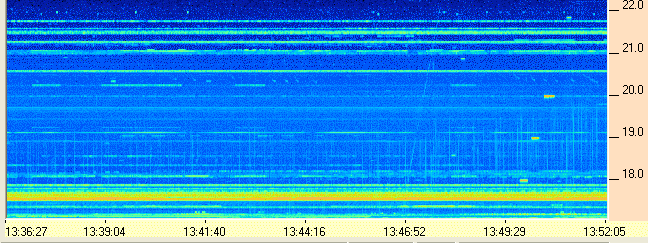
\includegraphics[width=8cm]{images/01}
\caption{Decametric Radio Emissions \citep{ashcraft13}}
\label{fig:dam_Emissions}
\end{figure}
%

Data collected by the two Voyager spacecraft in 1979 \citep{belcher87} and the later Galileo mission in 1995 \citep{kivelson96} added hugely to the understanding of the plasma interactions between Jupiter and Io and the source of the \gls{DAM} emissions. It was discovered that the Io has a thin atmosphere made up of a number of neutral gasses namely sodium, potassium, sulphur, and oxygen as shown in Figure. \ref{fig:io_neutral_gasses}. It is generally thought these gasses have been emitted through volcanic activity on the surface of the moon \citep{belcher87}. The gasses in orbit of Io have a very short life time, due to collisions with magnetospheric electrons. This gives rise to a plasma torus (\gls{IPT}) which co-rotates with Jupiter itself \citep{belcher87}. This can also be seen in Figure. \ref{fig:io_neutral_gasses} which shows the \gls{IPT}.

%
\begin{figure}[here]
\centering
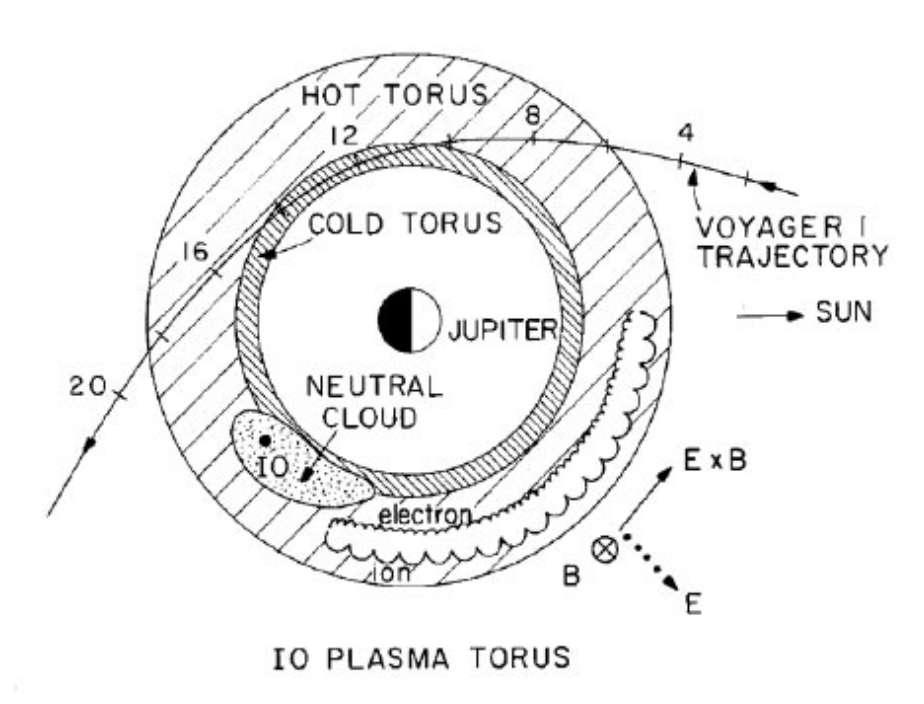
\includegraphics[width=8cm]{images/02}
\caption{Neutral Gasses in Orbit of Io \citep{belcher87}}
\label{fig:io_neutral_gasses}
\end{figure}
%

%
\newglossaryentry{IPT}
{
  name={IPT},
  description={Io Plasma Torus is created by Jovian atmospheric electrons ionizing neutral atmospheric gas such as sulphur in orbit around Io},
  sort=IPT
}
%

%
\newglossaryentry{IFT}
{
  name={IFT},
  description={Io Flux Tube is a cylindrical area of space containing magnetic field lines},
  sort=IFT
}
%

%
\begin{figure}[here]
\centering
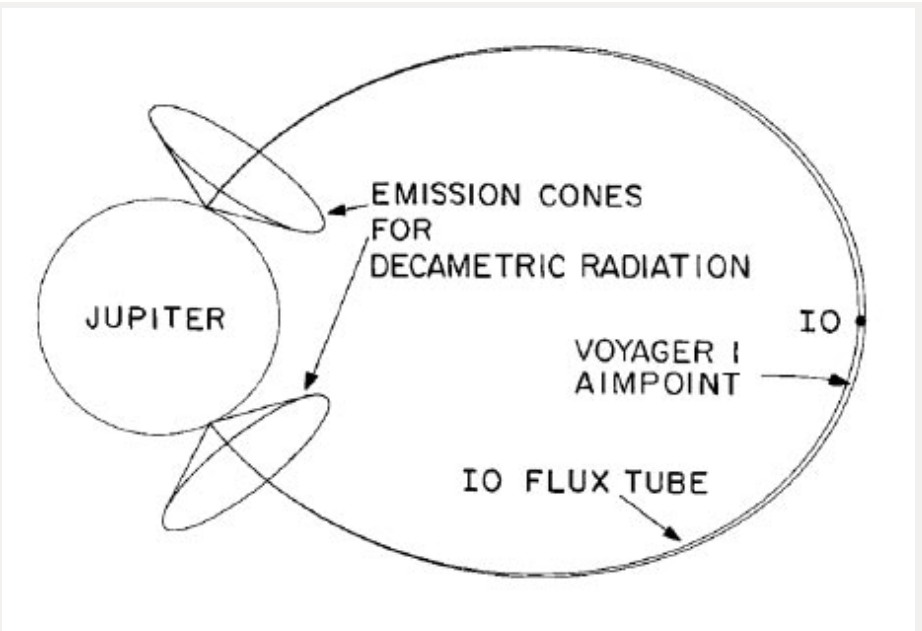
\includegraphics[width=6cm]{images/03}
\caption{Magnetic Flux Tube linking Jupiter and its satellite Io \citep{belcher87}}
\label{fig:io_flux_tube}
\end{figure}
%

The local co-rotation speed of the plasma torus is faster than the Keplerian orbit of the moon, and the plasma overtakes Io in its orbit at \begin{math} 57 km\;s^{-1} \end{math} \citep{belcher87}. Figures \ref{fig:io_flux_tube} and \ref{fig:io_flux_tube_plasma_torus} detail diagrams of the Io Flux Tube (\gls{IFT}) which is a cylinder shaped tube of space containing Jovian magnetic field lines \citep{belcher87} which link Io to Jupiter's ionosphere at both poles. A large portion of the decametric emissions come from the area where this \gls{IFT} meets the Jovian ionosphere \citep{belcher87}. 

As Io orbits within this flux torus it acts as a unipolar conductor \citep{bose08}, and Alfv\'en waves are regularly produced which carry an electric charge along the magnetic field lines between Io and Jupiter \citep{bose08}.

These Alfv\'en waves reflect between Jupiter's ionosphere at both north and south poles and Io up to 9 times \citep{bose08} while following Io through its orbit, thereby acting as a standing wave \citep{bose08}. It appears the source of the \gls{DAM} emissions are largely due to these reflections of the Alfv\'en waves off Jupiter's ionosphere in both the northern and southern regions \citep{bose08}. See Figure. \ref{fig:io_plasma_torus} which shows the Alfv\'en wings reflecting from Jupiter's Ionosphere creating emission cones.

The \gls{DAM} emissions radiate outwards in the shape of a cone as show in Figure. \ref{fig:io_flux_tube} \citep{belcher87}. When Io is at specific points in its orbit of Jupiter, these emission cones are pointing in the direction of Earth, at which point emissions can be picked up at ground based radio telescope listening stations.

%
\begin{figure}[here]
\centering
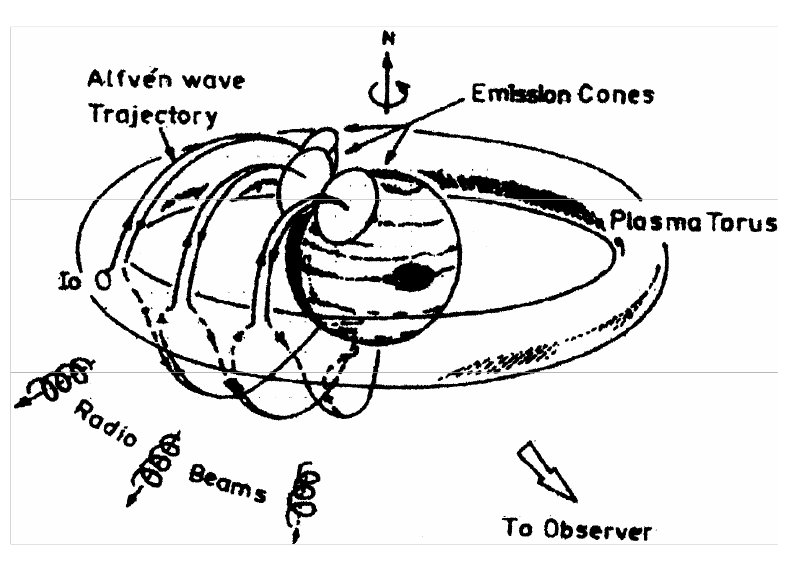
\includegraphics[width=8cm]{images/04}
\caption{Alfv\'en Waves following Io through its orbit and the DAM Emission cones \citep{bose08}}
\label{fig:io_plasma_torus}
\end{figure}
%

%
%%%%%%%%%%%%%%%%%%%%%%%%%%%%%%%%%%%%%%%%%%%%%%%%%%%%%%%%%%%%%%%%%%%%%%%%%%%%%%%%%%%%%%%%%%%
%
%\newpage
%\section*{Research Topic}
%\addcontentsline{toc}{section}{Research Topic}
%Students should identify whether the research outcomes are likely to have universal application or have a defined scope. This is important in gauging the extent to which the work is capable of independent replication.
%

%
\newglossaryentry{WRC}
{
  name={WRC},
  description={World Radio Communication Conference},
  sort=WRC
}
%

%
\newglossaryentry{HF}
{
  name={HF},
  description={High Frequency},
  sort=HF
}
%

A ground based listening station aiming to record \gls{DAM} emissions from Jupiter is most likely to succeed between 15-25 MHz \citep{wilkinson94}. According to \cite{arrl-00} there is no clear definition of the \textit{shortwave} radio bands however it is most often considered to extend from 3 MHz to 30 MHz. ComReg is the Irish Commission for Communications Regulation within Ireland, and maintains a list of the short wave frequencies which are designated for transmission purposes in Ireland and can be seen in Figure. \ref{fig:irish_electromagnetic_transmission_ranges} \citep{comreg14}.

%
\begin{figure}[here]
\centering
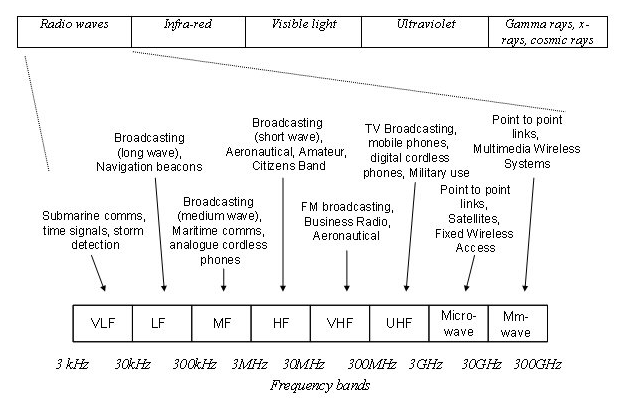
\includegraphics[width=8cm]{images/06}
\caption{Irish Regulatory Transmission Ranges \citep{comreg14}}
\label{fig:irish_electromagnetic_transmission_ranges}
\end{figure}
%

As many commercial short wave radio stations transmit in the lower end of the high frequency (\gls{HF}) 3-7 MHz range, it can be extremely busy and potentially difficult to monitor \gls{DAM} emissions where they are strongest. Amateur Radio operators also operate frequently in mid-late \gls{HF} ranges (\textit{160m, 80m, 60m, 40m, 30m, 20m, 17m, 15m, 12m and 10m bands}) while the higher frequency \gls{DAM} emissions taper off in strength very quickly. This limits the potential listening range significantly. Despite these obstacles, there are sections of the \gls{HF} spectrum which are suitable to capture Jovian emissions. One frequency to monitor Jovian \gls{DAM} emissions which is recommended by the Radio Jove project is \textit{20.1 MHz} \citep{nasa12}. 

Sourcing a suitable antenna is one of the first requirements to satisfy in order to capture \gls{DAM} emissions. Antennas are generally best suited to collect electromagnetic radiation at single specific frequencies, but may resonate and therefore operate over a range of frequencies depending on the design \citep{nasa12}. The wavelength ($\lambda$) which corresponds with the frequency (\textit{f}) \textit{20.1 MHz} can be obtained using the wavelength equation as shown in fig \ref{fig:wavelength_equation}. The corresponding wavelength for the frequency \textit{20.1 MHz} works out to be \textit{14.925 m} using this equation.

%
\begin{figure}[here]
  \centering
  \begin{equation}  	
    \lambda = \frac{c}{f}
  \end{equation}
  \begin{equation}
    \lambda = \frac{3\times10^8 m/s}{20.1\times10^6 Hz} = 14.925373134328359 m
  \end{equation}
  \caption{Wavelength Equation}
  \label{fig:wavelength_equation}
\end{figure}
%

One simple antenna design for collecting \gls{DAM} emissions is the \textit{dipole}. A dipole antenna can be constructed simply and cheaply from two pieces of wire and three insulators \citep{nasa12}, while ensuring to cut the wires to a length matching half the desired wavelength being captured \citep{nasa12}. However as the formula referenced in Figure. \ref{fig:wavelength_equation} describes the use of an \textit{infinitely thin} wire which is not possible in reality, \textit{capacitive end effects} must be taken into account when working out the resonating wavelength for a dipole antenna \citep{nasa12}.

The formula for calculating the resonating frequency for a half wavelength dipole is described in fig \ref{fig:wavelength_equation_dipole} and produces the value which should measure from tip to tip on the wires used to construct the dipole antenna \citep{nasa12}. \cite{RSGB-14} states in practice that the true resonance is not exactly multiples of the half-wavelength due to factors such as the coatings on the wire and loss due to radiation. A second formula is detailed in Figure. \ref{fig:wavelength_equation_wire_antenna} which takes these factors into account and produces an antenna length which is slightly larger than the formula proposed by \citep{nasa12}. Formula. 4 \textit{n} stands for the number of half-wavelengths in the antenna.

%
\begin{figure}[here]
  \centering
  \begin{equation}  	
    \bigg(\frac{\lambda}{2}\bigg)m = \frac{142.65}{20.1 MHz} = 7.097014925373134 m
  \end{equation}
  \caption{Wavelength Equation for Real World Half Wavelength Dipole Antenna}
  \label{fig:wavelength_equation_dipole}
\end{figure}
%

%
\begin{figure}[here]
  \centering
  \begin{equation}  	
    \lambda m = 155 \bigg(\frac{n - 0.05}{f}\bigg)
  \end{equation}
  \begin{equation}  	
    \lambda m = 155 \bigg(\frac{1 - 0.05}{20.1 MHz}\bigg)  = 7.325870646766169 m
  \end{equation}
  \caption{Wavelength Equation for Real World Half Wavelength Wire Antenna}
  \label{fig:wavelength_equation_wire_antenna}
\end{figure}
%

The radio emissions come in several different forms each with slightly different characteristics. Table. \ref{tab:dam_emissions} shows a list of the more widely known types which can be picked up using ground based listening equipment, and also has some information about their different characteristics \citep{wilkinson94}. Any particular observation session might be made up of some or all of these different types of \gls{DAM} emission and can last from a few minutes to several hours for larger noise storms \citep{wilkinson94}.

%
\begin{table}
  \centering
  \begin{tabular}[pos]{| c | c | c |}
    \hline
    Type & Emission Length & Emission Description\\ \hline
    S-Bursts & short generally 1-10 milliseconds & wideband bursts, several MHz wide\\ \hline
    L-Bursts & long 0.5 - 5 seconds & wideband bursts, several MHz wide\\ \hline
    N-Bursts & milliseconds upto seconds & narrowband bursts, several kHz wide\\
    \hline
  \end{tabular}
  \caption{Most common types of DAM Emissions from Jupiter \citep{wilkinson94}}
  \label{tab:dam_emissions}
\end{table}
%

Figure. \ref{fig:dam_emissions_spectrum} shows an ideal case of the \textit{S-Burst} and \textit{L-Burst} \gls{DAM} emissions and what they might look like on a frequency spectrum graph. S-Burst emissions are short, generally $1-10x10^{-3}s$ long while L-Bursts can be \textit{0.5-5s} in length.

%
\begin{figure}[here]
\centering
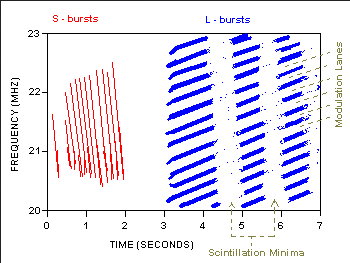
\includegraphics[width=8cm]{images/05}
\caption{Ideal DAM Emissions types from Jupiter \citep{wilkinson94}}
\label{fig:dam_emissions_spectrum}
\end{figure}
%

%%%%%%%%%%%%%%%%%%%%%%%%%%%%%%%%%%%%%%%%%%%%%%%%%%%%%%%%%%%%%%%%%%%%%%%%%%%%%%%%%%%%%%%%%%%
%
\newpage
\section*{Research Hypothesis}
\addcontentsline{toc}{section}{Research Hypothesis}
%
\newglossaryentry{SDR}
{
  name={SDR},
  description={Software Defined Radio is the creation of radio functions within software rather than hardware},
  sort=SDR
}

The aim of this project is to design and construct a low cost, self sufficient software defined radio (\gls{SDR}) telescope listening station, which can capture signals for transmission to a central data aggregation point for signal processing and analysis. This telescope should be suitable to study signals  in the \gls{DAM} (10-100 m) band at or near the \textit{20.1 MHz} frequency in order to pick up emissions produced by either Jupiter or the Sun.

There are a number of challenges which need to be overcome to achieve this, such as Jupiter only being visible for a number of months each year and then generally in the evening, night, or morning hours. Often at highly unsociable times. For this reason a radio telescope listening site should be as automated as possible.

%
\begin{figure}[here]
\centering
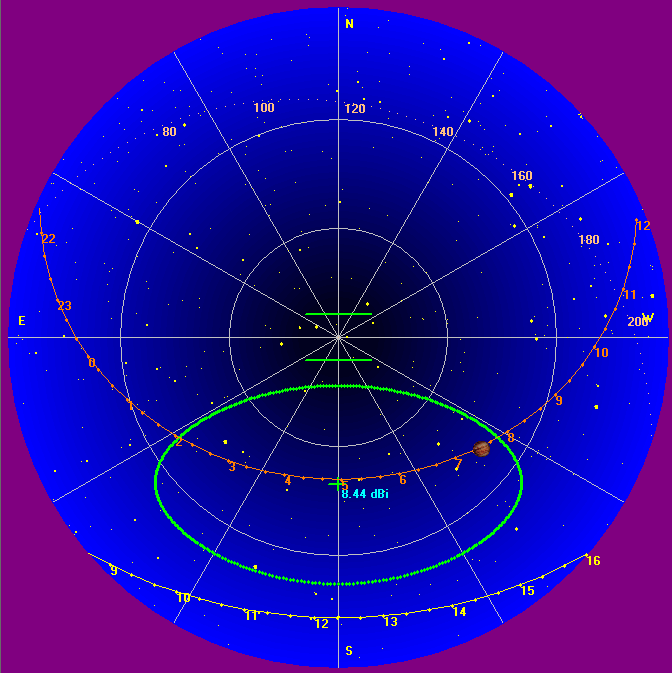
\includegraphics[width=8cm]{images/07}
\caption{Dual Dipole Antenna Beam at 20FT and 135deg phasing South \citep{nasa12}}
\label{fig:dual_dipole_20ft_135phasing_s}
\end{figure}
%

During daylight hours, the ionosphere becomes opaque to signals in the \gls{DAM} band due to becoming ionised by solar radiation \citep{nasa-ionosphere-12}. The proposed system will have a short window in the order of 1-6 hours every second night and early morning or so during which it may be possible to capture \gls{DAM} emissions from Jupiter. The Sun is a source of \gls{DAM} emissions also, and the telescope can capture solar storm emissions without modification, providing the Sun passes through the antenna beam. The telescope may require manual reconfiguration in order to pick up solar storm emissions during the day.


%
\begin{figure}[here]
\centering
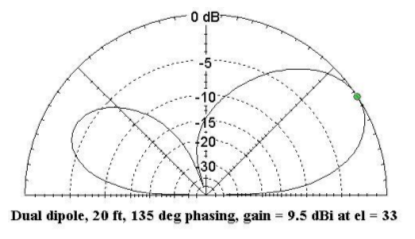
\includegraphics[width=8cm]{images/09}
\caption{Dual Dipole Antenna Array Beam\citep{nasa12}}
\label{fig:dual_dipole_antenna_array_beam}
\end{figure}
%

Interference from human sources such as short wave radio stations or amateur radio operators are also likely to affect the collection of \gls{DAM} emissions from Jupiter. The ability for automated flagging or removal of interference would be a desirable feature of the system. Lightning storms can also produce interference which will affect observations, it might be desirable for the system to handle natural interference sources also.

%
\begin{figure}[here]
\centering
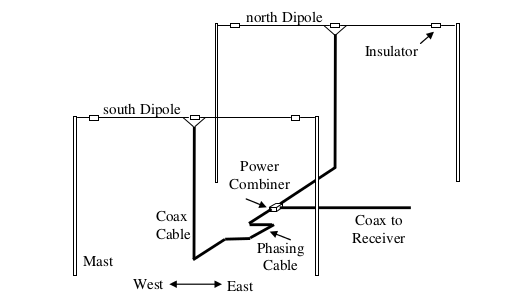
\includegraphics[width=8cm]{images/08}
\caption{Dual Dipole Antenna Array \citep{nasa12}}
\label{fig:dual_dipole_antenna_array}
\end{figure}
%

%This should outline the approach and methodology being proposed by the student to address the research question.
\newpage
\section*{Methodology}
\addcontentsline{toc}{section}{Methodology}
The section aims to provide a summary of the methodologies which will be followed on this project in order to answer the research questions put forward in the next section. It is broke up into the following subsections:

\begin{description}
  \item[Antenna Build] \hfill \\
    Building the antenna is further broken down into the following steps:
    \begin{itemize}
      \item source materials to build a dual dipole antenna
      \item build the telescope antenna
      \item validate the antenna is capable of collecting signals at or near the 20.1 MHz frequency \\
    \end{itemize}
  \item [Analysis of Listening Site Suitability] \hfill \\
    Finding a site suitable to deploy the antenna will require a site survey with the antenna connected to a spectrum analyser.
    \begin{itemize}
      \item source a spectrum analyser suitable for performing a site survey
      \item perform the survey at this site
      \item repeat until suitable site is found 
      \item deploy the antenna at a site \\
    \end{itemize}
  \item [Data Collection] \hfill \\
    Jupiter is visible above the horizon at night only during certain periods see Figure. \ref{fig:dual_dipole_antenna_array_beam}. In order to perform the required data collection it is highly desirable to automate the process if possible.
    \begin{itemize}
      \item create listening schedule during which \gls{DAM} emissions are likely to occur using the Radio Jove software
      \item develop \gls{SDR} prototype mechanism for gathering raw data from the antenna\\
    \end{itemize}
  \item [Data Analysis] \hfill \\
    Collected data can be analysed manually at first in order to validate the testbed, but later using software such as the development of basic algorithms to spot events such as \textit{S-Bursts} occurring in the data.
    \begin{itemize}
      \item analyse data collected for evidence of Jovian or Solar \gls{DAM} emissions
      \item analyse data for evidence of interference from human sources
      \item analyse data for evidence of interference from natural sources
      \item develop a system which connects to the dxspider server and creates flag events for human identified emissions at or near the target frequency being monitored by the telescope
      \item develop a system which interacts with the Blitzortung servers and creates flag events for emissions generated by lightning \\
    \end{itemize}
  \item [Data Processing] \hfill \\
    \gls{SDR} data processing techniques can be developed in order to better filter the signals as they are being collected thereby minimising the level of processing at a later stage.
    \begin{itemize}
      \item using \gls{SDR} techniques, to reduce interference in data as it is being collected
      \item attempt to remove instances of human and natural interference using signal processing techniques after collection \\
    \end{itemize}
  \item [Data Aggregation] \hfill \\
    An API layer allows 3rd parties the ability to access data collected from multiple listening sites and potentially develop new features or systems using the data.
    \begin{itemize}
      \item develop API layer to allow external parties access aggregated data collected by the system \\
    \end{itemize}
  \item [Design Platform] \hfill \\
    An analysis of the current available \gls{IOT} technologies and some of the available options which could be used in order to produce an open low cost platform which amateur astronomers could use in order to study emissions in the \gls{DAM} band.
    \begin{itemize}
      \item design a self sufficient automated platform suitable for collection of signals such as those by the \gls{SDR} telescope \\
    \end{itemize}
\end{description}

The \gls{SDR} hardware transceiver used is likely to be the \textit{HackRF} system while the \gls{SDR} software components will be developed in either \textit{C++} or \textit{Python} as both languages have bindings for the \textit{GNURadio} development tool-kit \citep{gnuradio-14}. The backend aggregation system with API will most likely be developed in the \textit{Ruby} language as this language is highly expressive and suitable for rapid prototype development. Execution of the Ruby application on the Java VM is capable using the \textit{JRuby} system, which will also allow the incorporation of any required Java libraries.


\subsection*{Potential Pitfalls}
%Predecisions on how I want to collect data, creating the research questions

It is difficult to determine at this early stage what will ultimately prove to be the most troublesome element to implement, however there are a number of potential pitfalls which have already been identified.

%
\begin{figure}[here]
\centering
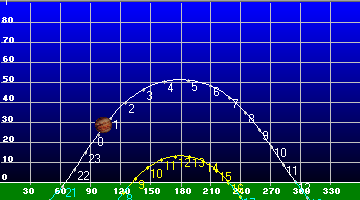
\includegraphics[width=8cm]{images/11}
\caption{Radio Jove graph showing Jupiter's max altitude 2014 \citep{rjp-14}}
\label{fig:jupiter_max_altitude_2014}
\end{figure}
%

The latitude of Ireland is 53.3$^{\circ}$ degrees N. In Ireland Jupiter reaches a maximum altitude of 52$^{\circ}$ degrees in 2014 see Figure. \ref{fig:jupiter_max_altitude_2014}. The telescope configuration which will be documented will apply only to locations at this or a similar latitude. It will be universally applicable at this latitude without modification throughout the world, and with relatively minor modifications to the configuration of the antenna it can be used at all locations. \cite{nasa12}

The \gls{SDR} complexity of the solution required in order to correctly filter interference might ultimately prove too resource intensive to work with a low power system such as the \textit{Raspberry Pi} or \textit{Beaglebone Black}. It might become apparent that the minimum system requirements may need to be increased to an \textit{Intel Atom} powered Netbook for example, or potentially something a lot more powerful such as an \textit{i3} or \textit{i5} system. If this was the case, it will drastically increase the power and cost requirements of the system should it be self sufficient, requiring bigger batteries, more capable/expensive photovoltaic and or wind turbines to keep the system topped up.



%
%%%%%%%%%%%%%%%%%%%%%%%%%%%%%%%%%%%%%%%%%%%%%%%%%%%%%%%%%%%%%%%%%%%%%%%%%%%%%%%%%%%%%%%%%%%
%
\newpage
\section*{Research Questions}
\addcontentsline{toc}{section}{Research Questions}
%A clear, precise definition of the problem is very important to focus on the research activity. great care should be used in devising the research questions. They define the structure of the investigation/innovation that will be used and an essential metric of the quality of the dissertation is the degree to which the research question has/have been answered.
The initial research questions which arise are as follows:

%
\newglossaryentry{IOT}
{
  name={IOT},
  description={Internet of Things a buzzword for everything connecting to everything},
  sort=IOT
}

\newglossaryentry{IQ}
{
  name={IQ},
  description={Imaginary Quadrature signal - Complex signal data and quadrature phase values in a digital signal sample},
  sort=IQ
}
%

\begin{enumerate}
  \item \textit{What current Internet of Things (\gls{IOT}) technologies would best suit the development of a software defined radio signal listening station and how cheaply can it be created?}
  \begin{itemize}
  	\item How feasible to use wireless technologies such as Zigbee, WIFI or Bluetooth to stream collected data to a central facility?
  	\item If wireless technologies prove too slow, is 10/100/1000 MBit Ethernet suitable instead? Or link aggregation technologies such as EtherChannel or LACP.
  	\item Can a low powered computing platform such as the Raspberry Pi 2B or Beaglebone Black be used to host the system, or will a more powerful system be required?
  \end{itemize}
  
  \item \textit{What processes or algorithms need to be developed to filter or flag known instances of human radio interference from radio signal observations?}
  \begin{itemize}
  	\item Flag transmission signals identified by amateur radio enthusiasts from a local DXSpider server in recorded data.
  	\item Flag instances of natural radio interference such as lightning from the Blitzortung server in recorded data.
  \end{itemize}
  
  \item \textit{What \gls{SDR} processes and algorithms need to be developed to identify instances of the three main \gls{DAM} emission types detailed in Table. \ref{tab:dam_emissions}?}
  \begin{itemize}
  	\item Can existing signal demodulation techniques be employed to find \gls{DAM} emissions?
  	\item What is required from an algorithm which might identify \gls{DAM} emissions within an \gls{IQ} signal?
  \end{itemize}
  
\end{enumerate}

%
%%%%%%%%%%%%%%%%%%%%%%%%%%%%%%%%%%%%%%%%%%%%%%%%%%%%%%%%%%%%%%%%%%%%%%%%%%%%%%%%%%%%%%%%%%%
%
\newpage
\section*{Literature Review}
\addcontentsline{toc}{section}{Literature Review}
%This should contain a review of a number of books, journal articles and web references of relevance to the research area proposed. The literature should contain seminal and recent referenced research material that is categorised under a number of relevant sub-themes.

The literature review can be broken down into the following areas:


\begin{itemize}
  \item[\textbullet] What are the decametric radio emissions and what are they caused by
  \item[\textbullet] Potential radio telescope designs which could be replicated in order to collect DAM emissions
  \item[\textbullet] Digital signal processing
\end{itemize}

\subsection*{Decametric Radio Emission what are they and where do they come from?}
\cite{belcher87} states that the data collected by both \textit{Voyager} spacecraft fit with the Alfv\'en wing theory as an explanation for the source of the \gls{DAM} emissions \citep{belcher87}. \cite{kivelson96} discusses the refinements made to this theory to take into account the flowing plasma between Jupiter's ionosphere and the electrically conducting Io. The \textit{Galileo} spacecraft collected data which appears to corroborate the updates to the Alfv\'en wing model \citep{kivelson96}. \cite{bose08} states that the Alfv\'en waves reflect off Jupiter's ionosphere which cause the \gls{DAM} emissions to radiate out from the point in Jupiter's ionosphere where it meets the \gls{IFT} in a cone shape. \cite{imai-08} proposes an update to this model to take into account the decade long shifts in \gls{DAM} emission patterns, and proposes an extension to the emission cone model to include a \textit{searchlight} shaped emission zone \citep{imai-08} see Figure. \ref{fig:decametric_emissions_searchlight}.

\subsection*{Radio Telescope Designs, Which to Choose?}
The NASA project \textit{Radio Jove} recommended the dual dipole array design for a cheap low cost listening site as shown in Figure. \ref{fig:dual_dipole_antenna_array} \citep{nasa12}. But it is by no means the only antenna design which would be capable of picking up the \gls{DAM} emissions. \cite{wilkinson94} recommends a slightly more advanced design, the \textit{folded dipole} which maximises the bandwidth available to the antenna \citep{wilkinson94}. \cite{greef-12} details a third alternative for collecting \gls{DAM} emissions, a shortwave loop antenna as can be seen in Figures. \ref{fig:loop_antenna_design_a}, \ref{fig:loop_antenna_design_b} and \ref{fig:loop_antenna_design_c}.

\subsection*{Digital Signal Processing}
\cite{smith-03-a} explains that digital signal processing is a term used to describe the mathematics, algorithms and techniques used to manipulate signals after they have been converted from analogue to digital. \cite{freidt-13} holds that digital signal processing is the preferred means to process signals, for reasons such as stability and for its resistance to long term ageing effects that analogue systems suffer from. However as \cite{smith-03-b} points out, due to the nature of the conversion from analogue to digital, information is lost in this process. \cite{smith-03-b} maintains that the proper sampling of an analogue signal occurred if you can reconstruct the signal from the digital samples collected, and incorrect sampling will lead to loss of the original signal due to aliasing.

%
\begin{figure}[here]
\centering
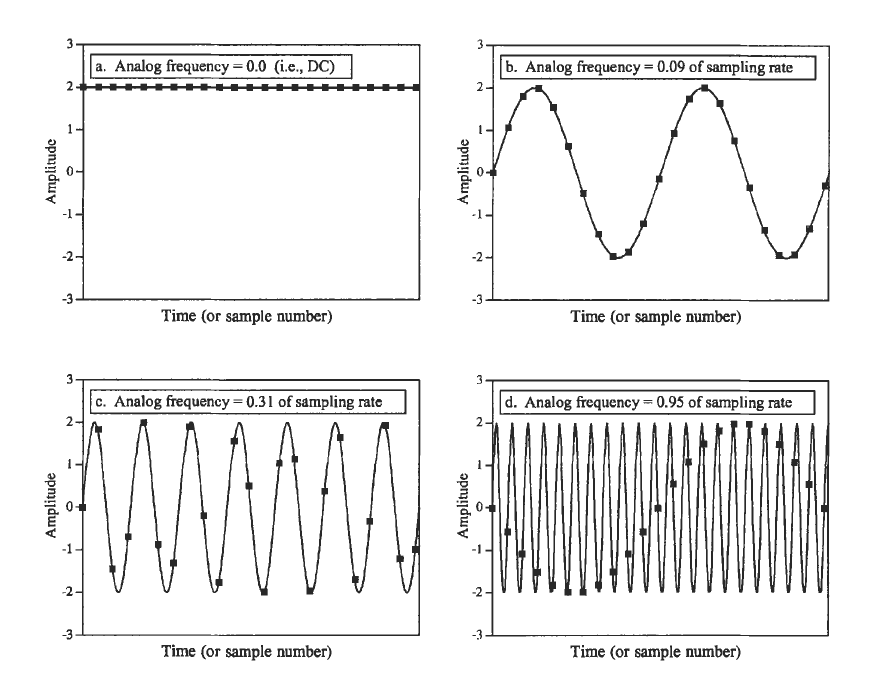
\includegraphics[width=8cm]{images/44}
\caption{Sampling an Analogue Signal \citep{smith-03-b}}
\label{fig:smith_sample_theorem_2003}
\end{figure}
%

\cite{smith-03-b} demonstrates in Figure: \ref{fig:smith_sample_theorem_2003} how signal data loss occurs due to aliasing. When sampling an analogue signal which has a frequency more than half of the sample rate (Nyquist frequency), \cite{smith-03-b} observes that the original signal cannot be reconstructed. This is referred to as the sampling theorem \citep{smith-03-b} where $f_s$ is the sample rate and $f$ is the frequency being sampled.

%
\begin{figure}[here]
  \centering
  \begin{equation}  	
    f_s > 2f
  \end{equation}
  \caption{Sampling Theorem aka Nyquist-Shannon sampling theorem \citep{smith-03-b}}
  \label{fig:nyquist-shannon-sample-theorem}
\end{figure}
%

\cite{ossmann-15-b} contends that the application of Nyquist-Shannon sampling theorem only applies to real analogue signals where the bandwidth is equal to half the sample rate. However for a complex digital signal  the bandwidth is equal to the sample rate \citep{ossmann-15-b}.

Due to the cheap availability of computational resources, digital signal processing is capable of being carried out now within software entirely, this has led to the development of software defined radio solutions \citep{freidt-13}. The GNURadio software allows creation of software defined radio solutions by replacing hardware functions with modular software functions. These software functions are capable of being connected together, an output from one function providing input for another. It is in this fashion it is possible to transform digital signals using digital signal processing methods within the GNURadio platform\citep{gnuradio-14}.

%
\begin{figure}[here]
\centering
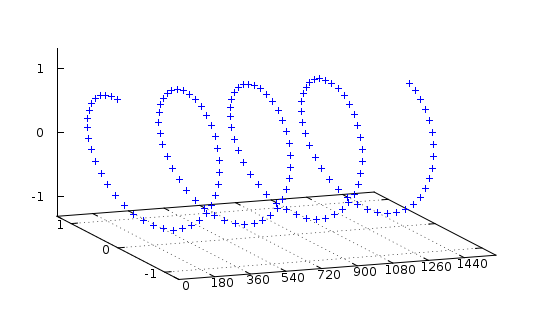
\includegraphics[width=7cm]{images/48}
\caption{I/Q Samples Helix \citep{kuisma-14}}
\label{fig:kuisma-iq-helix}
\end{figure}
%

\cite{ossmann-15-a} illustrates how the HackRF One \gls{SDR} transceiver can be accessed within GNURadio by way of the osmocomm source which is an abstraction layer between GNURadio and the HackRF driver. Figure: \ref{fig:ossmann_am_demodulation} shows an amplitude modulation signal which has been digitally sampled. In order to demodulate such a signal, an understanding how the signal data is stored is a must. Digital periodic signal samples tend to be stored in a complex format which amounts to polar coordinates \citep{ossmann-15-c}. $I$ is the point on the real axis, and $Q$ is an angle which contains the imaginary component. See Figure: \ref{fig:kuisma-iq-helix} shows how these I/Q values are plotted periodically and Figure: \ref{fig:kuisma-iq-polar} shows the I/Q polar data \citep{kuisma-14}.

%
\begin{table}
  \centering
  \begin{tabular}{ | p{2.5cm} || p{2.5cm} | p{2.5cm} | p{2.5cm} | p{2.5cm} |}
    \hline
    \textbf{Topic} & \textbf{Belcher 1987} & \textbf{Kivelson et al 1996} & \textbf{Bose et al 2008} & \textbf{Imai et al 2008} \\ \hline \hline
    What are the Jovian DAM emissions and what causes them? & Large fraction of DAM emissions come from point where IFT meets Jupiter's ionosphere (p3). Large moving conductor within a magnetised plasma (p1) produces Alfv\'en wing. & Alfv\'enic disturbances, generated by flowing plasma from Jovian magnetosphere and conducting Io (p337). & Alfv\'en waves reflecting off Jupiter's Ionosphere (p79). & Not fully understood, but believed to be produced by cyclotron maser instability \citep{imai-08}. \\ \hline \hline

    \textbf{Topic} & \textbf{Wilkinson et al 1994} & \textbf{NASA Radio Jove 2012} & \textbf{Greef 2012} &  \\ \hline \hline

    Radio telescope designs suitable to capture DAM emissions from Jupiter & Wilkinson et al suggest a folded dipole antenna design & Radio Jove project suggest a dual dipole antenna & Greef demonstrates a low cost Loop Antenna design with reflection plate & \\ \hline \hline
    
    \textbf{Topic} & \textbf{Smith 2003} & \textbf{Freidt 2013} & \textbf{GNU Radio 2014} & \textbf{Ossmann 2015} \\ \hline \hline    
    
    Digital signal processing & Smith argues digital signal processing is one of the most powerful technologies that will shape the 21st century. & Freidt states digital signal processing now ubiquitous, and cheap availability of computational power lends self to software defined radio solutions. & GNURadio allows digital signal processing using transformation functions developed in software. & Ossmann argues that the HackRF One is perfectly suited as a low cost wide range transceiver for use within software defined radio prototypes. \\
    \hline
  \end{tabular}
  \caption{Literature Review Synthesis Matrix}
  \label{tab:literature_review_synthesis_matrix}
\end{table}
%



%
%%%%%%%%%%%%%%%%%%%%%%%%%%%%%%%%%%%%%%%%%%%%%%%%%%%%%%%%%%%%%%%%%%%%%%%%%%%%%%%%%%%%%%%%%%%
%
%\newpage
%\section*{Description of the Experimental Design / Validation Methodology}
%\addcontentsline{toc}{section}{Description of the Experimental Design / Validation Methodology}
% A dissertation must employ rigorous scientific argument. The experimental design and the validation methodology must be specified in great detail in the proposal. At this proposal stage you should define clear evaluation criteria.


%\begin{itemize}
%  \item Identify data caused by lightning
%  \item Identify data caused by human emissions
%  \item Perform a site survey with the spectrum analyser
%  \item Replicate the testbed at a second site
%\end{itemize}

%
%%%%%%%%%%%%%%%%%%%%%%%%%%%%%%%%%%%%%%%%%%%%%%%%%%%%%%%%%%%%%%%%%%%%%%%%%%%%%%%%%%%%%%%%%%%
%
p
\newpage
\section*{Main Milestones Anticipated}
\addcontentsline{toc}{section}{Main Milestones Anticipated}
% Students should agree a number of milestones and their likely delivery dates with their supervisor at the start of the progress.

The following Table. \ref{tab:milestones_anticipated} details the milestones which have been identified and agreed to date. It has been updated for the Interim Report to include completed milestones and those in progress:

%
\begin{table}
  \centering
  \begin{tabular}{ | p{2cm} | p{2cm} | p{2cm} | p{5cm} |}
    \hline
    Deadline & Start & End & Summary \\ \hline \hline
    Antenna Build & October 14 & March 15 & Settle on a design for the telescope, source the parts for the build
    and finally construct the prototype antenna which will act as a template for the second dipole. \\ \hline
    Site Survey & March 15 & March 15 & Perform a site survey using a spectrum analyser connected to the prototype antenna. \\ \hline
    Deploy Dual Dipole Antenna & March 15 & March 15 & Deploy the antenna array at a suitable location and begin to collect data for analysis. \\ \hline
    Interim Report & January 15 & (Hard Deadline) 30th April 15 & Poster presentation to review panel and supervisor on 19th May \\ \hline
    Data Collection & March 15 & July 15 & Once the antenna is deployed begin collecting data for analysis. \\ \hline
    Data Analysis and System Development & March 15 & July 15 & Develop analytical SDR tools to filter or flag interference. Develop algorithms to detect the various DAM emission. \\ \hline
    Evaluate IOT Technologies & January 15 & July 15 & Experiment with the various IOT technologies which could potentially be used to create a self sufficient listening array. \\ \hline
    Final Report Submission & June 15 & (Hard Deadline) September 15 & First draft to supervisor due in early June 15. Complete draft due 24th August. Final submission 4th September \\
    \hline
  \end{tabular}
  \caption{Milestones Anticipated}
  \label{tab:milestones_anticipated}
\end{table}
%

%
\begin{figure}[here]
	\centering
	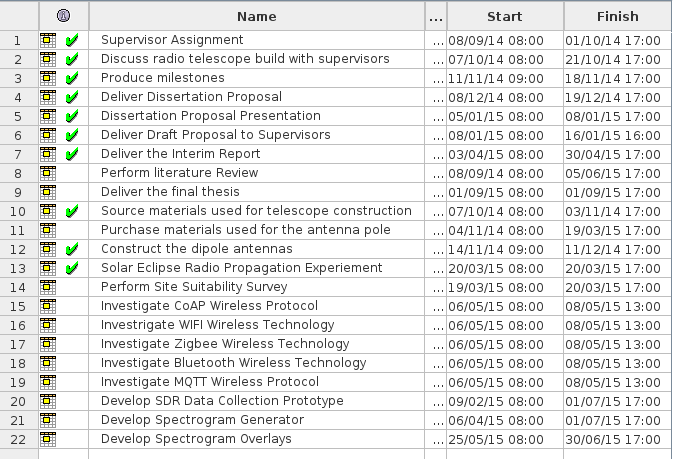
\includegraphics[width=9cm]{images/56}
	\caption{SDRT Gantt Chart Details}
	\label{fig:sdrt-gantt}
\end{figure}
%

%
\begin{figure}[here]
	\centering
	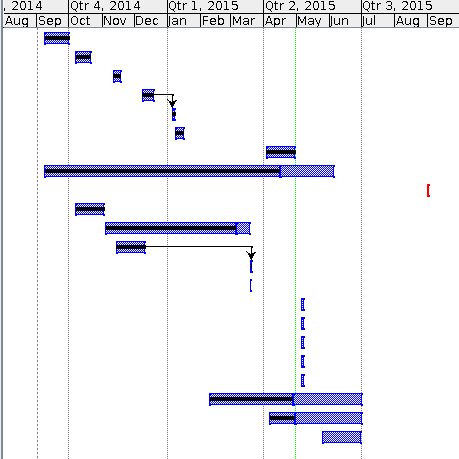
\includegraphics[width=9cm]{images/57}
	\caption{SDRT Gantt Chart}
	\label{fig:sdrt-gantt}
\end{figure}
%

%
%%%%%%%%%%%%%%%%%%%%%%%%%%%%%%%%%%%%%%%%%%%%%%%%%%%%%%%%%%%%%%%%%%%%%%%%%%%%%%%%%%%%%%%%%%%
%
\newpage
\chapter*{Testbed Build and Verification}
\addcontentsline{toc}{chapter}{Testbed Build and Verification}
The NASA Radio Jove dual dipole antenna design (Figure: \ref{fig:dual_dipole_antenna_array}) was chosen over the other designs for a number of reasons, namely:

\begin{itemize}
	\item Simplicity of the architecture and consequently also construction
	\item Low cost of building materials
	\item Reasonably effective performance (5-9 dB gain depending on configuration)
	\item Easy to operate and maintain
	\item Suitable for a permanent installation
	\item Large body of technical documentation supporting the operation
\end{itemize}


\section*{Special Resources Required}
\addcontentsline{toc}{section}{Special Resources Required}
% The research work may require access to specialised equipment, software, journals and so on.

The following resources have been identified as being required in order to perform the research and are listed as follows:

\begin{description}
  \item[GnuRadio] \hfill \\
  The GnuRadio software is an open-source software development tool kit that allows access to signal processing techniques in order to implement software radio solutions.
  \item[HackRF] \hfill \\
  The HackRF \gls{SDR} transceiver system is the software defined radio transceiver chosen for the prototype system.
  \item[PL259 / SO239] \hfill \\
  Cable adapters which connect coax cables together with the dipole center.
  \item[Radio Jove Software] \hfill \\
  The Radio Jove software is extremely useful for observers wishing to capture \gls{DAM} emissions from Jupiter. It contains a large number of features such as emission prediction observation charts, and information regarding Jupiter's location in the sky from any specified point on the Earth's surface.
  \item[RG59 Coax] \hfill \\
  RG59 coax cable is required to link the dipole antennas back to the \gls{SDR} transceiver.
  \item[Spectrum Analyser] \hfill \\
  A spectrum analyser will be required in order to perform a site survey to determine if a location is suitable for collecting \gls{DAM} emissions.
\end{description}


\section*{Antenna Build}
\addcontentsline{toc}{section}{Antenna Build}

\newglossaryentry{SWR}
{
  name={SWR},
  description={Standing Wave Ratio is the ratio of impedance between receiver and antenna},
  sort=SWR
}

In order to satisfy the main requirement of capturing \gls{DAM} signals at 20.1MHz construction of an antenna was needed. The equation shown in Figure: \ref{fig:wavelength_equation_wire_antenna} was used to calculate a starting estimate of the length of antenna wire required to construct this antenna. Many factors can affect the ability of an antenna to receive data at a particular frequency \citep{arrl-00}, such as the following:

\begin{itemize}
	\item quality of the wire conductor or thickness of the wire
	\item height that the antenna is mounted above the ground
	\item capacitive end effects
	\item closeness to radio conductors
\end{itemize}

One simple method of partly improving antenna performance is by controlling the length of the antenna wire while measuring the Standing Wave Ratio (\gls{SWR}) value, which is the ratio of impedance between the receiver and the antenna. The use of a \gls{SWR} analyser becomes invaluable in this process.

%
\begin{figure}[here]
\centering
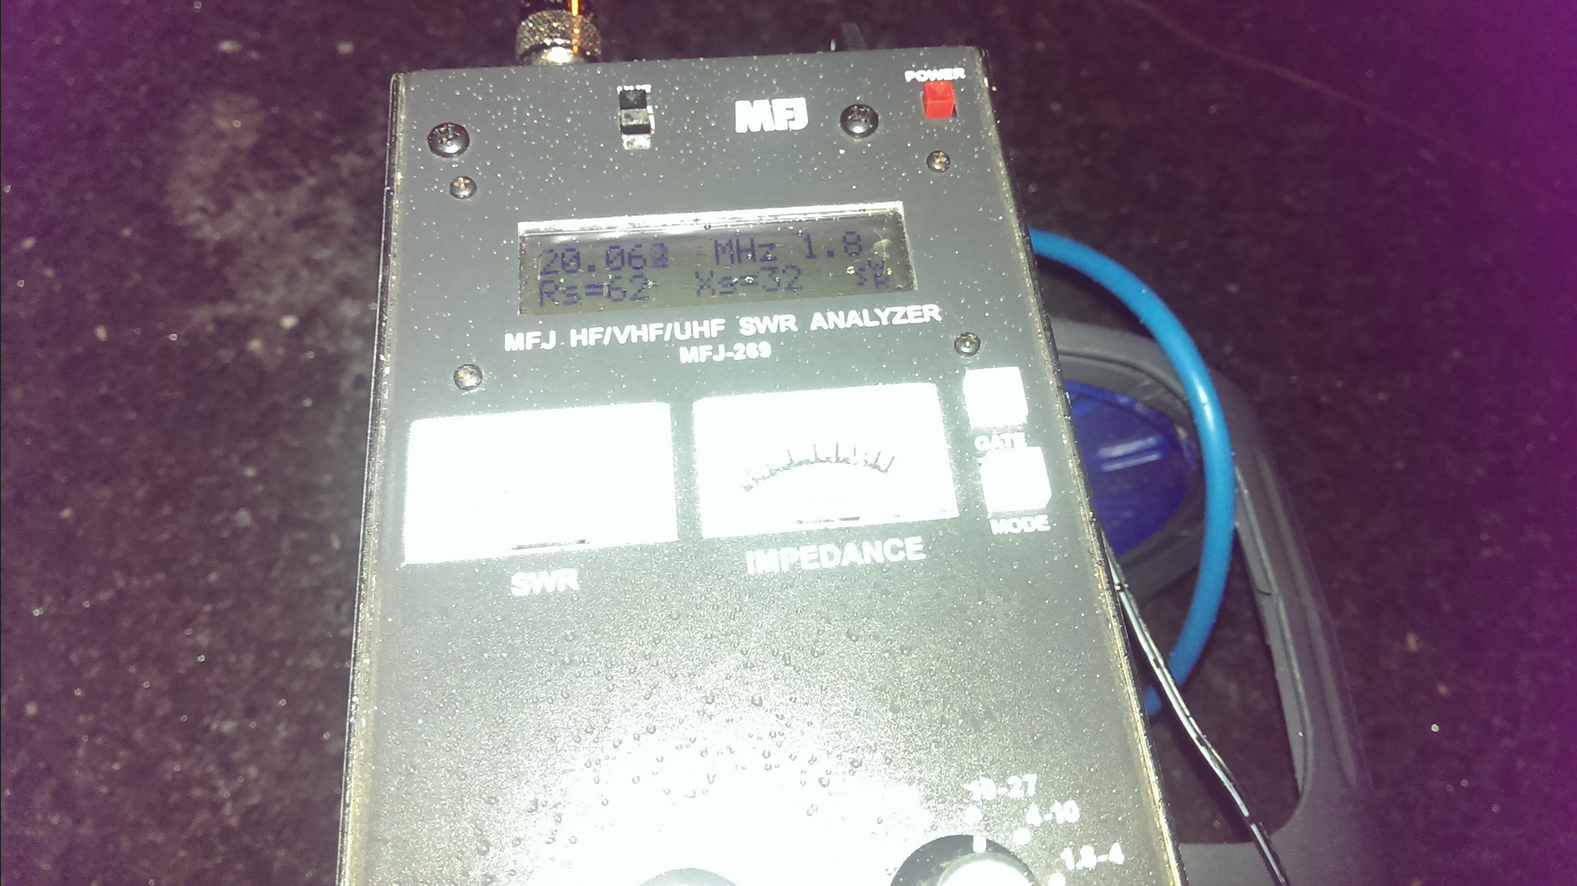
\includegraphics[width=8cm]{images/34}
\caption{Measuring the SWR of the antenna with an SWR Analyser}
\label{fig:swr_analyser_measuring_antenna}
\end{figure}
%

The initial length of antenna wire was cut to match the length produced by the equation in Figure: \ref{fig:wavelength_equation_wire_antenna} and was then cut in half before each end was connected to a dipole center. The antenna was placed on the ground before being connected to the \gls{SWR} analyser. The \gls{SWR} value for the antenna was measured, and it was discovered the antenna was suitable for capturing of signals at 18 MHz. The antenna was then shortened by a small identical amount on each side and the \gls{SWR} values were again measured until the antenna registered as being most suitable for operation at 20.1MHz as seen in Figure:  \ref{fig:swr_analyser_measuring_antenna}. 

The \gls{SWR} equations shown in Figure: \ref{fig:swr_equation} is the  equations where $|\rho|$ is the reflection coefficient, P$_{f}$ is the power in the forward wave entering the antenna while P$_{r}$ is the power of the reflected wave in the antenna \citep{arrl-00}.

%
\begin{figure}[here]
  \centering
  \begin{equation}
  	SWR = \frac{1 + |\rho|}{1 - |\rho|} 
  \end{equation}
  \begin{equation}
  	|\rho| = \frac{SWR - 1}{SWR + 1} 
  \end{equation}
  \begin{equation}
  	|\rho| = \sqrt{\frac{P_r}{P_f}}
  \end{equation}
  \caption{Standing Wave Ratio Equations}
  \label{fig:swr_equation}
\end{figure}
%

%
\begin{figure}[here]
  \centering
  \begin{equation}
  	|\rho| = \frac{1.2 - 1}{1.2 + 1} 
  \end{equation}
  \begin{equation}
  	|\rho| = 0.09090909090909088
  \end{equation}
  \begin{equation}
  	0.09090909090909088 = \sqrt{\frac{P_r}{100}}
  \end{equation}
  \begin{equation}
  	0.09090909090909088^2 = \frac{P_r}{100}
  \end{equation}
  \begin{equation}
  	P_r = 0.826446280991735
  \end{equation}
  \caption{Calculating P$_{r}$ for the antenna}
  \label{fig:swr_equation_pr}
\end{figure}
%

The value of \gls{SWR} for the antenna should be ideally as close as possible to 1, this ensures all the signal energy collected by the antenna is transferred to the load successfully. However in practice this is never the case as all antennas have varying amounts of loss. The antenna once mounted had a measured \gls{SWR} value of 1.2 which equates to a P$_{r}$ value as shown in Figure: \ref{fig:swr_equation_pr} of 0.826446280991735 which is a loss of 17.35\% or about 1dB which is considered reasonable \citep{arrl-00}.

\newpage
Table: \ref{tab:antenna_build_cost} gives a breakdown of the costs associated with the antenna build to date.

%
\begin{table}
  \centering
  \begin{tabular}{p{8cm} l}
    \toprule
    Item Name & Cost (\euro) \\ \midrule
    100m Copper Wire & 20.00  \\
    100m Coax RG59 & 25.00  \\
    2 $\times$ Dipole Centers & 20.00 \\
    8 $\times$ PL259 & 18.00 \\
    2 $\times$ SO239 & 4.00 \\
    SMA-SO239 Adapter & 4.50 \\
    2 $\times$ SO239-SO239 Adapter & 4.50 \\
    T Adapter & 3.00 \\
    Patch Lead & 5.00 \\
    2 $\times$ 4m 5cm Pipe & 15.00 \\
    2 $\times$ 4m 4cm Pipe & 15.00 \\
    \bottomrule
    \\
    Total & 134.00
  \end{tabular}
  \caption{Antenna Build Cost}
  \label{tab:antenna_build_cost}
\end{table}
%


\section*{Listening Site Suitability}
\addcontentsline{toc}{section}{Listening Site Suitability}
A convenient location for the antenna deployment was selected and the antenna was deployed. It was necessary to determine if this site was in fact a suitable location to host a radio telescope antenna. In order measure the ambient noise at the site, a Tektronics SA2600 spectrum analyser was connected to the antenna and left for 2 hours at midday to gather data. The spectrum is likely to be full of radio interference from human and natural sources at this time. The results can be seen in Figure: \ref{fig:site_survey_spec_analyser}. The ambient \gls{RF} noise at the site was quite high, ranging between -80dB and -70dB on average. 

\newglossaryentry{preamp}
{
  name={preamp},
  description={preamplifier - is an electronic amplifier that prepares a small electrical signal for further amplification or processing},
  sort=preamp
}

Similar readings were taken using the HackRF while attached to the antenna as show in Figure: \ref{fig:site_survey_hackrf}. The measurements recorded with the HackRF were performed using the \textit{gqrx} \gls{SDR} software while all amplification settings inside \textit{gqrx} were set at 0, in order to get an accurate reading on the raw signal being collected by the antenna. The values were on average -20dB quieter than those recorded by the SA2600 spectrum analyser, this points towards an inherent deafness flaw in the HackRF design itself, and possibly the requirement of a preamplifier (\gls{preamp}) in order to boost the gain on the input signal. 

\newglossaryentry{RF}
{
  name={RF},
  description={Radio Frequency},
  sort=RF
}

%
\begin{figure}[here]
\centering
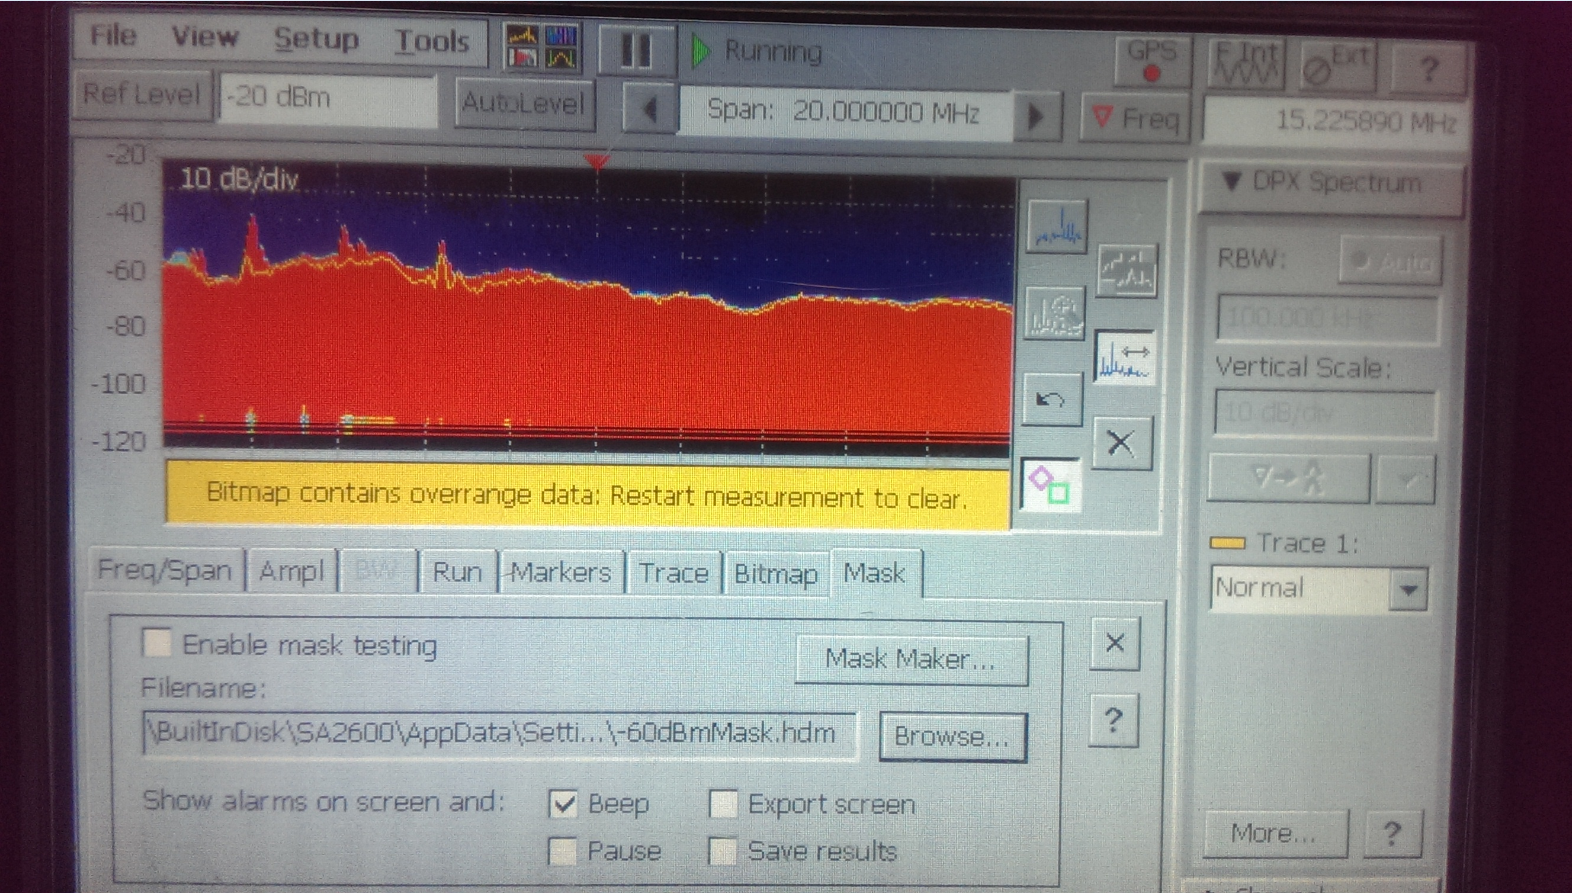
\includegraphics[width=8cm]{images/26}
\caption{Site Survey performed using a Tektronics SA2600 Spectrum Analyser}
\label{fig:site_survey_spec_analyser}
\end{figure}
%

%
\begin{figure}[here]
\centering
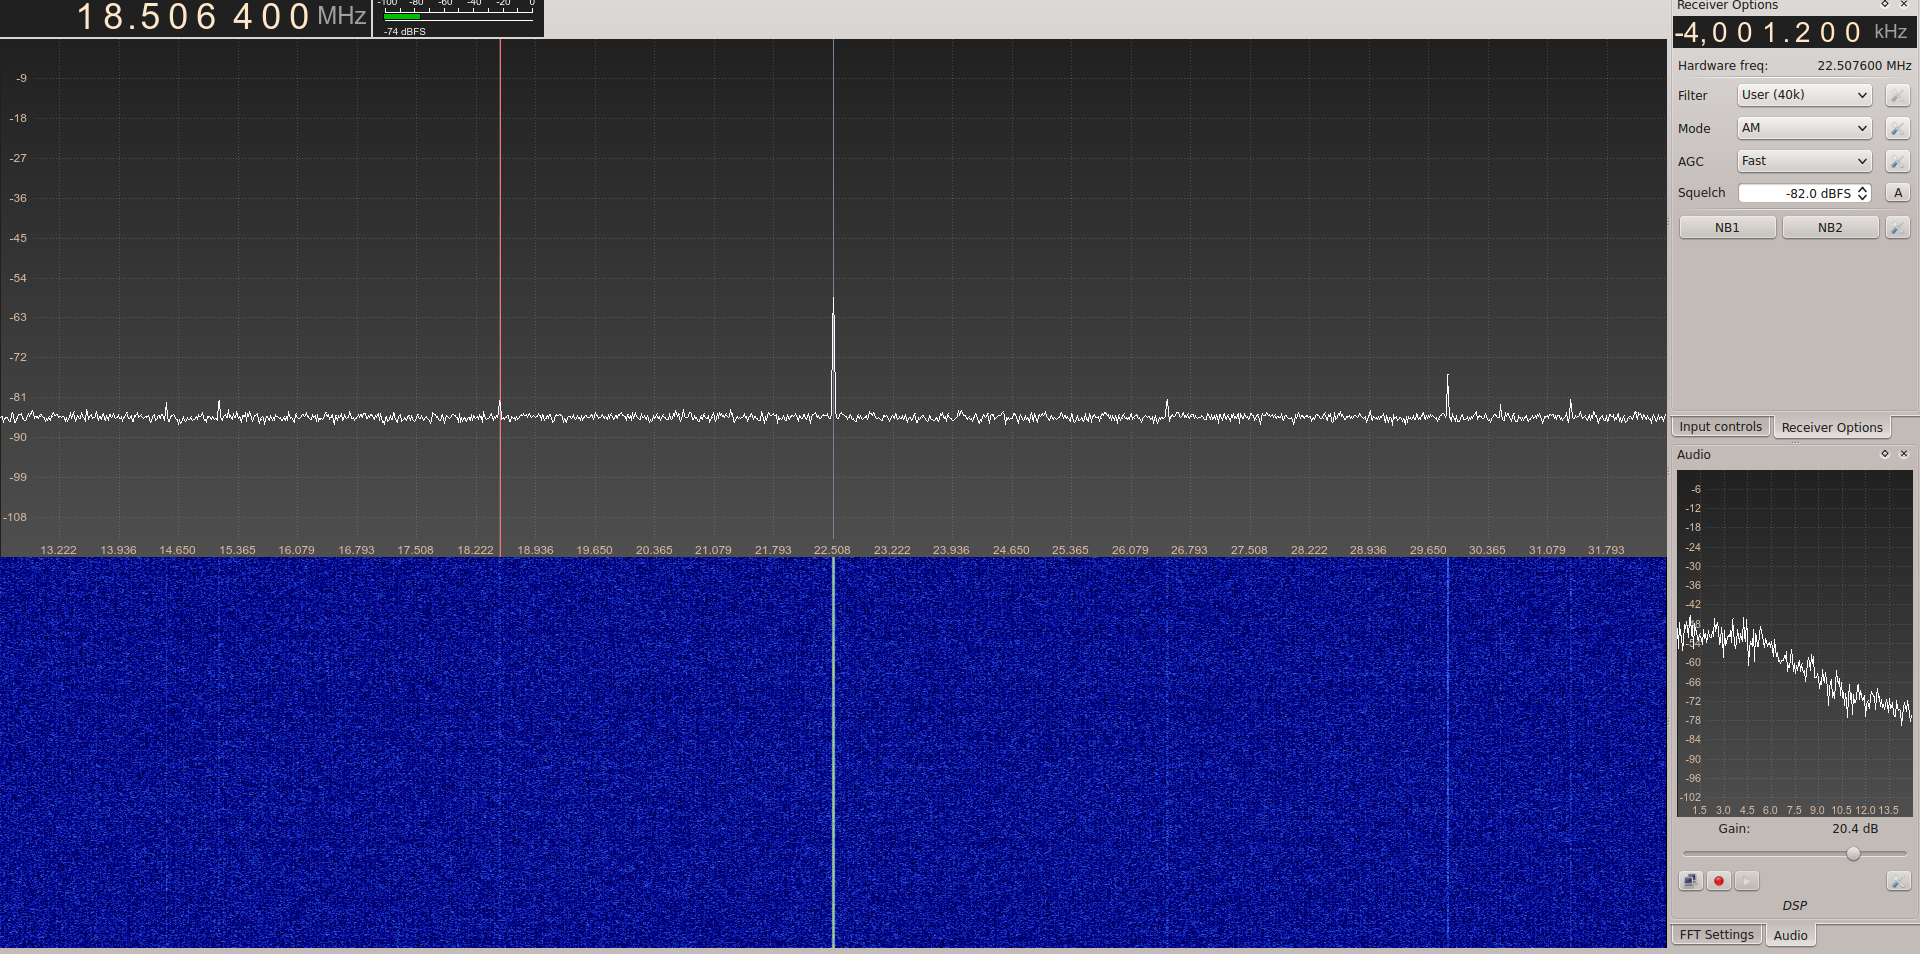
\includegraphics[width=8cm]{images/31}
\caption{Site Survey performed using HackRF One}
\label{fig:site_survey_hackrf}
\end{figure}
%

\newglossaryentry{LOFAR}
{
  name={LOFAR},
  description={Low Frequency Array - https://www.astron.nl/lofar-telescope/lofar-telescope},
  sort=LOFAR
}

In May 2013, the Solar Physics Group from Trinity College Dublin, performed a site survey at Birr Castle to assertain the suitability of the site for an installation of the Low Frequency Array (\gls{LOFAR}) telescope \citep{craf-13}. The study was focused on a wide range of frequencies between 10 and 400MHz, a portion of which can be seen in Figure: \ref{fig:site_survey_lofar}. The report concluded that the location at Birr Castle was a relatively quiet location as compared against a site at Bornim, Germany and another at Bleien, Switzerland. 

From the results of this survey, it can be seen that the average background noise levels were about -55dB near 20MHz which is similar to those recorded 80km away at the Kilkenny site. Table: \ref{tab:site_survey} details the results collected at the Kilkenny site and also includes those performed by the Solar Physics Group at Birr Castle for comparison. Results indicate the Kilkenny site appears to be a reasonable location at which to host the radio telescope.

%
\begin{figure}[here]
\centering
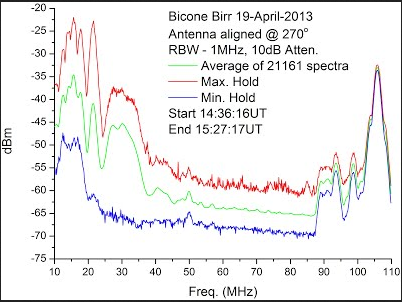
\includegraphics[width=8cm]{images/35}
\caption{LOFAR Site Suitability Survey performed at Birr Castle \citep{craf-13}}
\label{fig:site_survey_lofar}
\end{figure}
%

%
\begin{table}
  \centering
  \begin{tabular}{p{2cm} l r}
    \toprule
    Site & Equipment & Average Noise at 20.1MHz \\ \midrule
    Kilkenny & Tektronix SA2600 20.1MHz Dipole & -65dB  \\
    Kilkenny & HackRF One 20.1MHz Dipole & -65dB \\
    Birr & LOFAR Array 10-100MHz Schwarzbeck Bicone & -55dB \\
    \bottomrule
  \end{tabular}
  \caption{Average Noise Measurements at Kilkenny Listening Site compared to Birr Listening Site \citep{craf-13}}
  \label{tab:site_survey}
\end{table}
%

\newglossaryentry{RSGB}
{
  name={RSGB},
  description={RSGB - The Radio Society of Great Britain},
  sort=RSGB
}

\newglossaryentry{MW}
{
  name={MW},
  description={MW - Medium Wave frequencies usually in the wavelengths 300 kHz - 3 MHz},
  sort=RSGB
}

\section*{Verification of the Radio Receiver}
\addcontentsline{toc}{section}{Verification of the Radio Receiver}
An opportunity to validate the HackRF transceiver arose with the announcement of a public Medium Wave (\gls{MW}) experiment by \cite{RSGB-15-b} of the Radio Society of Great Britain (\gls{RSGB}). The \gls{RSGB} Propagation Studies Committee intended to perform an experiment during the partial solar eclipse on 20th March 2015. As can be seen in Figure: \ref{fig:solar_eclipse_scale}, the UK and Ireland would witness more than 90\% totality during the eclipse. This was an opportunity to perform simple experiments to demonstrate the Sun's effect on Earth's ionosphere, and how this ionisation affects the propagation of radio signals.

According to \cite{nichols-15-a}, \gls{MW} radio stations which are located more than 500 km away are unlikely to be propagated during daylight hours due to their signals being absorbed by the D layer as shown in Figure: \ref{fig:atmosphere_ionisation_effects_mw}. However this D layer does not exist during night time hours, as a result these radio signals are free to reflect from the E and F layers. \cite{RSGB-15-b} states that this is also true during a solar eclipse with a high totality percentage as would occur on the 20th March 2015.

\cite{RSGB-15-b} provided some a number of radio stations which transmit signals in the \gls{MW} range at various locations in the United Kingdom, Europe and also a number in Iceland. The experiment called for choosing a station which is transmitting in the \gls{MW} range and is also capable of being heard at the listeners location during the night time. This station should not be capable of being heard during the day time, the experiment called for a station which is further away than 500 km. The chosen radio station should then be tuned in to coincide with the beginning of the solar eclipse. The station receive power should be plotted against time. It was expected that the signal strength of the radio station should rise to a maximum which coincided with the solar eclipse maximum.


%
\begin{figure}[here]
	\centering
	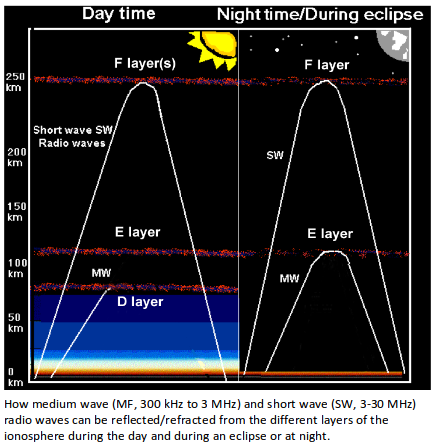
\includegraphics[width=8cm]{images/53}
	\caption{Comparing propagation of \gls{MW} radio signals during day and during night/solar eclipse \citep{RSGB-15-b}}
	\label{fig:atmosphere_ionisation_effects_mw}
\end{figure}
%

\subsection*{Methodology}
The following methodology was followed during this experiment:

\begin{enumerate}
	\item The dipole antenna built for use in the main part of the dissertation was not best suited for picking up signals in the \gls{MW} range so an alternative design was chosen. 
	\item A Beverage antenna was picked as it was easily aimed and had a simple design. The antenna very simply consisted of a copper wire 80 m long attached to a long wire antenna terminator which had an SO239 connector.
	\item The listening site was longest in the East-West axis, while the receiver was positioned at the far west end of the site. For this reason a radio station in the East.
	\item The antenna was aimed in the direction of the radio station chosen, and simply placed on the ground.
	\item HackRF was tuned to the chosen radio station.
	\item 2 MHz bandwidth of the spectrum was recorded during the entire length of the solar eclipse, the signal strength of the radio station can be plotted against time at a later date using this recorded data.
	\item The \gls{SDR} receiver should have the automatic gain control switch off in order to get accurate power results. 
\end{enumerate}

The chosen radio station was \textit{Radio China International} (1440 MHz) which was a powerful signal during the night time despite it being transmitted from Marnach in Luxembourg which is 950 km away from the listening site. The HackRF \gls{SDR} receiver was tuned to 1440 MHz and \gls{IQ} samples were recorded once the solar eclipse began. As the eclipse neared 10\% totality, the radio station began to emerge from the background noise which was -70 dB. The signal rose steadily until the eclipse maximum point which was -25 dB, and then slowly fell in signal strength once more as the totality value dropped. The results were submitted to \citet{RSGB-15-b} for inclusion in the overall experiment.

A number of issues with the HackRF \gls{SDR} transceiver became apparent during this experiment. The technical specifications show the operating range of the HackRF to be 10 MHz - 6 GHz \citep{ossmann-15-d}. In practice it is unreliable when tuning to frequencies below 4 MHz. This proved a problem as the frequency being monitored were at 1440 MHz. The HackRF appears to be quite deaf without maxing the IF and RF amplifiers. This could be solved by adding a \gls{preamp} at the antenna.


\section*{Capturing DAM Emissions}
\addcontentsline{toc}{section}{Capturing DAM Emissions}
Using the Radio Jupiter Pro software, a prediction was made that 23rd April 2015 would offer a very good opportunity to hear \gls{DAM} emissions. As can be seen in Figure: \ref{fig:dam_emissions_io_a_april_23_prediction}, at the point of the highest chance of capturing \gls{DAM} emissions, Jupiter was right on the very edge of the antenna beam focus. Due to the limitations in the design of the antenna, this configuration offered the best chance to receive an emission from Jupiter. 


%
\begin{figure}[here]
	\centering
	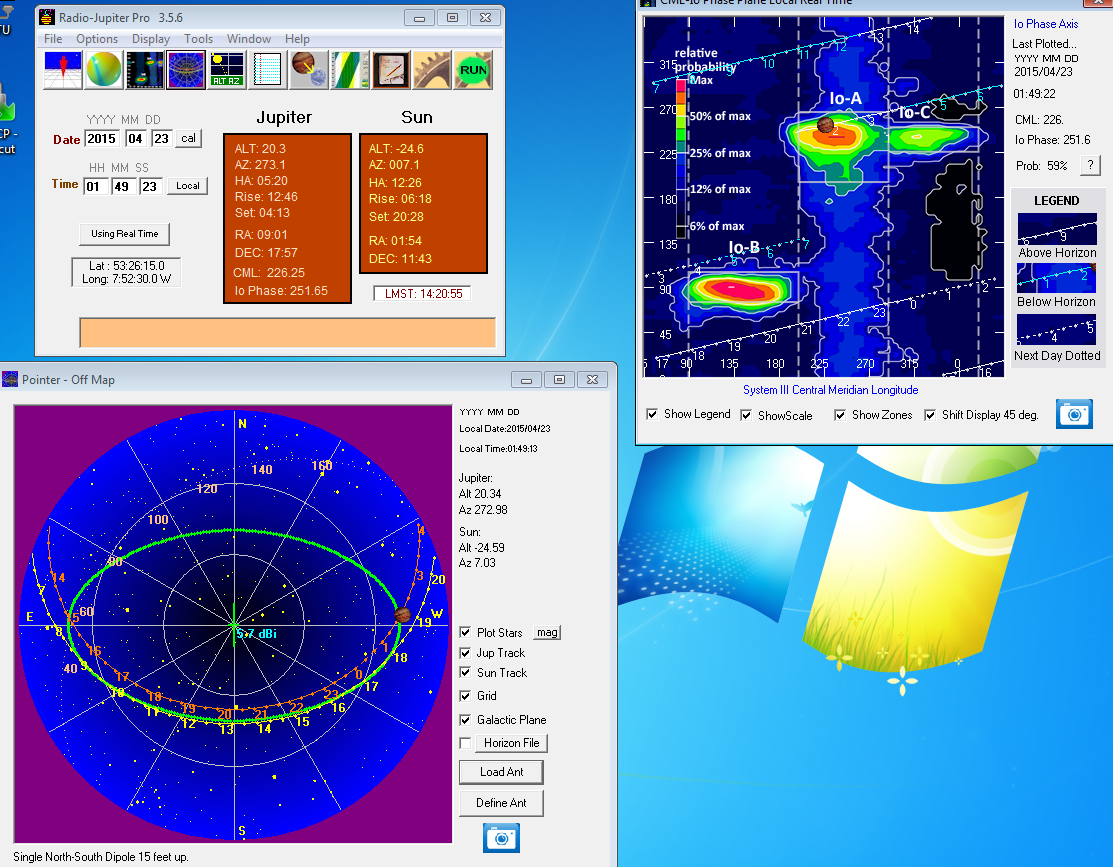
\includegraphics[width=8cm]{images/52}
	\caption{Jupiter \gls{DAM} IO-A Storm Prediction}
	\label{fig:dam_emissions_io_a_april_23_prediction}
\end{figure}
%

Despite this, a number of emissions were recorded as can be seen in in the raw image Figure: \ref{fig:dam_emissions_io_a_april_23}. The emissions appear as faint horizontal lines in this waterfall diagram. This diagram is limited by the small bandwidth of 2 MHz and short period of 2 minutes. Ideally in order to spot these interesting emissions a large bandwidth of 20 MHz for instance should be used, over a long period of observation such as 1-24 hours. An example of this is section of a spectrogram seen in Figure: \ref{fig:wide_radio_spectrogram}, which shows averaged signal power data for frequencies 17-55 MHz and 70-1000 MHz for a 24 hour period.

There are many open source software tools such as rtl\_power, simple\_ra and heatmap which could capture averaged raw signal strength data from a RTL based receiver in order to build spectrogram diagrams. Unfortunately most of this software is not compatible with the HackRF. However the basic functionality from these tools can be replicated using basic processing blocks within GNURadio and the spectrograms can be built using tools like Octave or Mathlab.

%
\begin{figure}[here]
	\centering
	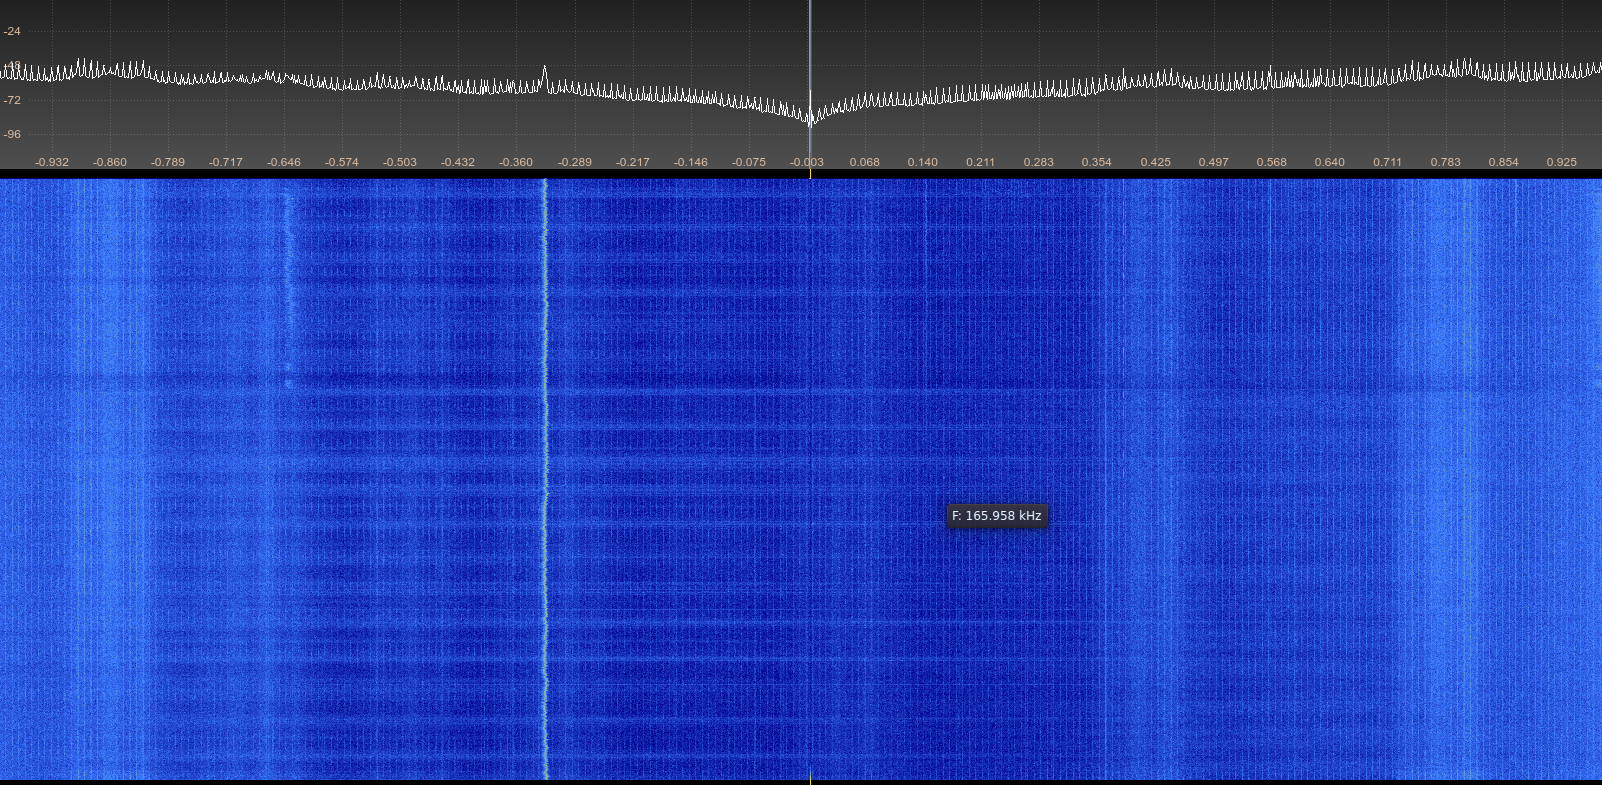
\includegraphics[width=8cm]{images/54}
	\caption{\gls{DAM} emissions picked up during an IO-A storm}
	\label{fig:dam_emissions_io_a_april_23}
\end{figure}
%

%
\begin{figure}[here]
	\centering
	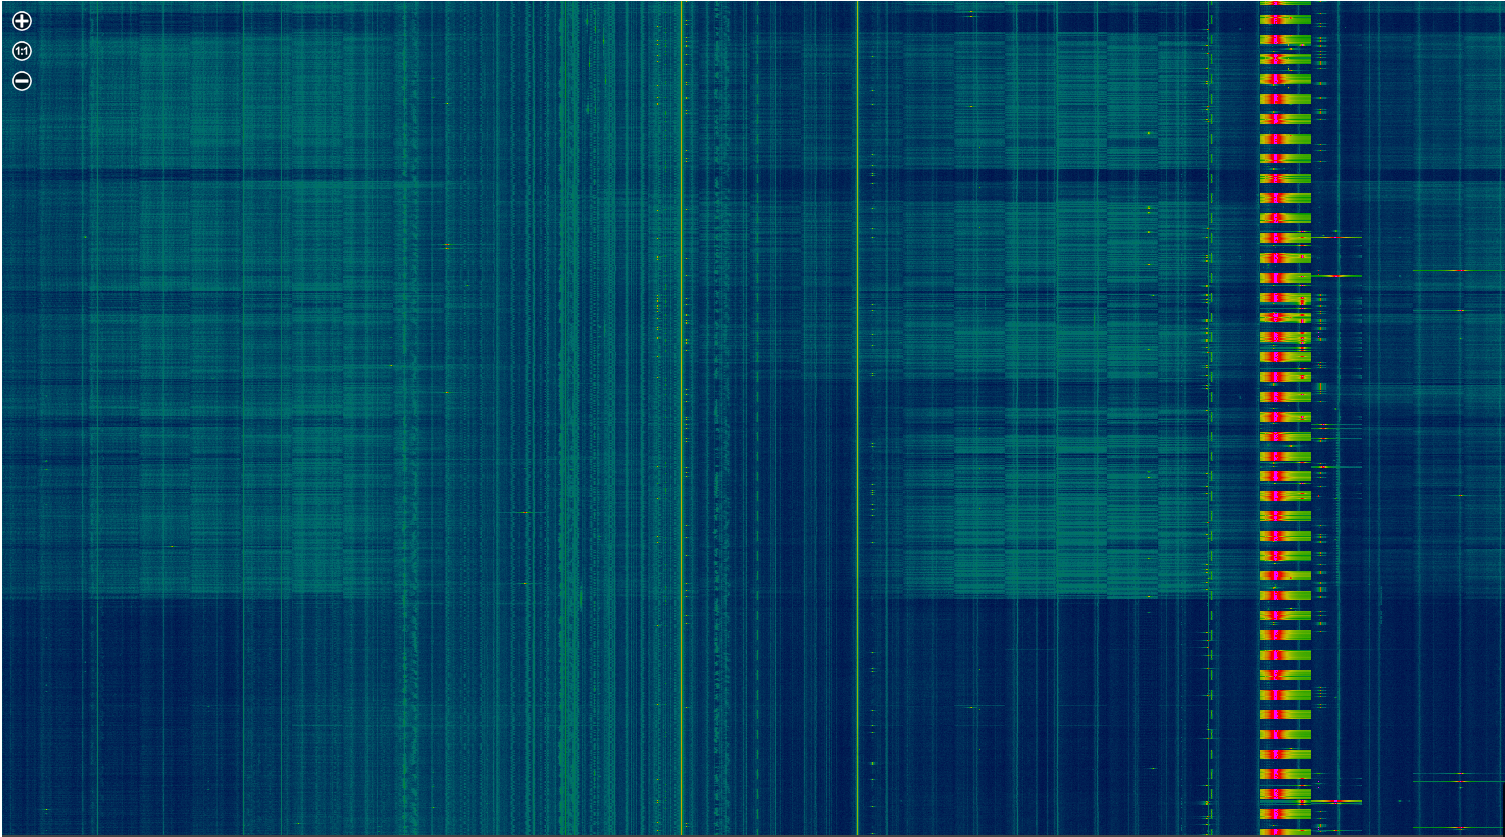
\includegraphics[width=8cm]{images/55}
	\caption{Radio Spectrogram Diagram \citep{superkuh-15}}
	\label{fig:wide_radio_spectrogram}
\end{figure}
%

% Background materials
% state of the art
% what I read up and needed to put it together
% research questions restated


% TODO Add some information about the data gathered to date.


%
%%%%%%%%%%%%%%%%%%%%%%%%%%%%%%%%%%%%%%%%%%%%%%%%%%%%%%%%%%%%%%%%%%%%%%%%%%%%%%%%%%%%%%%%%%%
%
\newpage
\chapter*{Research Question 1}
\addcontentsline{toc}{chapter}{Research Question 1}
% Chapter for each research question
% how we validated it and proved it worked

\textit{What current Internet of Things (\gls{IOT}) technologies would best suit the development of a software defined radio signal listening station and how cheaply can it be created?}

\begin{itemize}
  	\item How feasible to use wireless technologies such as Zigbee, WIFI or Bluetooth to stream collected data to a central facility?
  	\item If wireless technologies prove too slow, is 10/100/1000 MBit Ethernet suitable instead? Or link aggregation technologies such as EtherChannel or LACP.
  	\item Can a low powered computing platform such as the Raspberry Pi 2B or Beaglebone Black be used to host the system, or will a more powerful system be required?
\end{itemize}

While the work required to answer this research question is ongoing, it is expected it can be answered by performing a state of the art in this area and compare performance and cost analysis of the existing networking and storage technologies. The original proposal contained the desire to create a self sustaining listening site, renewable sources of energy and energy storage will also be considered.


\section*{Experiment 1}
\addcontentsline{toc}{section}{Determine SDRT Power Requirements}

%
\begin{table}
  \centering
  \begin{tabular}{p{2cm} l r}
    \toprule
    
    Site & Equipment & Average Noise at 20.1MHz \\
 & & \\
 & & \\
 \midrule
    Kilkenny & Tektronix SA2600 20.1MHz Dipole & -65dB  \\
    Kilkenny & HackRF One 20.1MHz Dipole & -65dB \\
    Birr & LOFAR Array 10-100MHz Schwarzbeck Bicone & -55dB \\
    \bottomrule
  \end{tabular}
  \caption{Average Noise Measurements at Kilkenny Listening Site compared to Birr Listening Site \citep{craf-13}}
  \label{tab:site_survey}
\end{table}
%





\subsection*{Methodology}
The following methodology was followed during this experiment:

\begin{enumerate}
	\item Aasdfasdf asdfasdfasdfasdf adsfasdf asdf s asdf  asdfadsfasdf. 
\end{enumerate}


\section*{Experiment 2}
\addcontentsline{toc}{section}{Experiment 2}
asdfasdf asdfasdf asdfasdfasdfasdf asdfasdf. asdfasdfasdfasdf asdfasdf asdfasdf asdfasdfasdfasdf asdfasdf. asdfasdfasdfasdf. asdfasdfasdfasdfasdfasdf asdfasdf. asdfasdf. asdfasdfasdfasdf asdfasdf asdfasdf asdfasdfasdfasdf asdfasdf. asdfasdfasdfasdf. asdfasdfasdfasdfasdfasdf asdfasdf. asdfasdf. asdfasdfasdfasdf asdfasdf asdfasdf asdfasdfasdfasdf asdfasdf. asdfasdfasdfasdf. asdfasdfasdfasdfasdfasdf asdfasdf. asdfasdf. asdfasdfasdfasdf asdfasdf asdfasdf asdfasdfasdfasdf asdfasdf. asdfasdfasdfasdf. asdfasdfasdfasdfasdfasdf asdfasdfasdfasdf. asdfasdfasdfasdf asdfasdf asdfasdf asdfasdfasdfasdf asdfasdf. asdfasdfasdfasdf. asdfasdfasdfasdfasdfasdf asdfasdf.


\subsection*{Methodology}
The following methodology was followed during this experiment:

\begin{enumerate}
	\item Aasdfasdf asdfasdfasdfasdf adsfasdf asdf s asdf  asdfadsfasdf. 
\end{enumerate}



\section*{Experiment 3}
\addcontentsline{toc}{section}{Experiment 3}
asdfasdf asdfasdf asdfasdfasdfasdf asdfasdf. asdfasdfasdfasdf asdfasdf asdfasdf asdfasdfasdfasdf asdfasdf. asdfasdfasdfasdf. asdfasdfasdfasdfasdfasdf asdfasdf. asdfasdf. asdfasdfasdfasdf asdfasdf asdfasdf asdfasdfasdfasdf asdfasdf. asdfasdfasdfasdf. asdfasdfasdfasdfasdfasdf asdfasdf. asdfasdf. asdfasdfasdfasdf asdfasdf asdfasdf asdfasdfasdfasdf asdfasdf. asdfasdfasdfasdf. asdfasdfasdfasdfasdfasdf asdfasdf. asdfasdf. asdfasdfasdfasdf asdfasdf asdfasdf asdfasdfasdfasdf asdfasdf. asdfasdfasdfasdf. asdfasdfasdfasdfasdfasdf asdfasdfasdfasdf. asdfasdfasdfasdf asdfasdf asdfasdf asdfasdfasdfasdf asdfasdf. asdfasdfasdfasdf. asdfasdfasdfasdfasdfasdf asdfasdf.


\subsection*{Methodology}
The following methodology was followed during this experiment:

\begin{enumerate}
	\item Aasdfasdf asdfasdfasdfasdf adsfasdf asdf s asdf  asdfadsfasdf. 
\end{enumerate}

%
%%%%%%%%%%%%%%%%%%%%%%%%%%%%%%%%%%%%%%%%%%%%%%%%%%%%%%%%%%%%%%%%%%%%%%%%%%%%%%%%%%%%%%%%%%%
%
\newpage
\chapter*{Research Question 2}
\addcontentsline{toc}{chapter}{Research Question 2}
% Chapter for each research question
% how we validated it and proved it worked

\textit{What processes or algorithms need to be developed to filter or flag known instances of human interference from radio signal observations?}

\begin{itemize}
	\item Flag transmission signals identified by amateur radio enthusiasts from a local DXSpider server in recorded data.
  	\item Flag instances of natural radio interference such as lightning from the Blitzortung server in recorded data.
\end{itemize}

A DX server is a system which Amateur (Ham) Radio operators may use in order to inform one another in real time, about instances of radio signal transmissions from DX stations and other amateur radio stations. These DX Servers are often connected together to form a cluster. This allows many users from all over the world to communicate and share this information by connecting to the cluster. It is a rich source of identified human transmissions which often have the time, location and signal frequencies which were recorded. The data being shared is also often rigidly structured which greatly simplifies the task of implementing a software parsing solution \citep{koopman-07}. 

A software client could be developed which might connect to a local DX Server and gather data related to transmissions within the frequency range currently being monitored by the telescope. When signals have been identified as being within the range they will be flagged and all related meta data will be stored for processing at a later stage.

The Blitzortung project operates an online service which displays global information about instances of lightning strikes in real time. \cite{blitzortung-14} provide the designs for a listening station which amateur enthusiasts can then build and operate. Each site can then share the information back to a central server in real time \citep{blitzortung-14}. A software client could be developed which might connect to this Blitzortung server and retrieve occurrences of lightning strikes within a certain range such as 500 km centred on the listening site.

It is envisioned the time and frequency values associated with this data related to human signals, along with the data gathered regarding lightning strikes could be used to generate an overlay for a waterfall spectrogram diagram of the previous 24 hours worth of data collected by the telescope.


\section*{Experiment 1}
\addcontentsline{toc}{section}{Experiment 1}
asdfasdf asdfasdf asdfasdfasdfasdf asdfasdf. asdfasdfasdfasdf asdfasdf asdfasdf asdfasdfasdfasdf asdfasdf. asdfasdfasdfasdf. asdfasdfasdfasdfasdfasdf asdfasdf. asdfasdf. asdfasdfasdfasdf asdfasdf asdfasdf asdfasdfasdfasdf asdfasdf. asdfasdfasdfasdf. asdfasdfasdfasdfasdfasdf asdfasdf. asdfasdf. asdfasdfasdfasdf asdfasdf asdfasdf asdfasdfasdfasdf asdfasdf. asdfasdfasdfasdf. asdfasdfasdfasdfasdfasdf asdfasdf. asdfasdf. asdfasdfasdfasdf asdfasdf asdfasdf asdfasdfasdfasdf asdfasdf. asdfasdfasdfasdf. asdfasdfasdfasdfasdfasdf asdfasdfasdfasdf. asdfasdfasdfasdf asdfasdf asdfasdf asdfasdfasdfasdf asdfasdf. asdfasdfasdfasdf. asdfasdfasdfasdfasdfasdf asdfasdf.


\subsection*{Methodology}
The following methodology was followed during this experiment:

\begin{enumerate}
	\item Aasdfasdf asdfasdfasdfasdf adsfasdf asdf s asdf  asdfadsfasdf. 
\end{enumerate}


\section*{Experiment 2}
\addcontentsline{toc}{section}{Experiment 2}
asdfasdf asdfasdf asdfasdfasdfasdf asdfasdf. asdfasdfasdfasdf asdfasdf asdfasdf asdfasdfasdfasdf asdfasdf. asdfasdfasdfasdf. asdfasdfasdfasdfasdfasdf asdfasdf. asdfasdf. asdfasdfasdfasdf asdfasdf asdfasdf asdfasdfasdfasdf asdfasdf. asdfasdfasdfasdf. asdfasdfasdfasdfasdfasdf asdfasdf. asdfasdf. asdfasdfasdfasdf asdfasdf asdfasdf asdfasdfasdfasdf asdfasdf. asdfasdfasdfasdf. asdfasdfasdfasdfasdfasdf asdfasdf. asdfasdf. asdfasdfasdfasdf asdfasdf asdfasdf asdfasdfasdfasdf asdfasdf. asdfasdfasdfasdf. asdfasdfasdfasdfasdfasdf asdfasdfasdfasdf. asdfasdfasdfasdf asdfasdf asdfasdf asdfasdfasdfasdf asdfasdf. asdfasdfasdfasdf. asdfasdfasdfasdfasdfasdf asdfasdf.


\subsection*{Methodology}
The following methodology was followed during this experiment:

\begin{enumerate}
	\item Aasdfasdf asdfasdfasdfasdf adsfasdf asdf s asdf  asdfadsfasdf. 
\end{enumerate}



\section*{Experiment 3}
\addcontentsline{toc}{section}{Experiment 3}
asdfasdf asdfasdf asdfasdfasdfasdf asdfasdf. asdfasdfasdfasdf asdfasdf asdfasdf asdfasdfasdfasdf asdfasdf. asdfasdfasdfasdf. asdfasdfasdfasdfasdfasdf asdfasdf. asdfasdf. asdfasdfasdfasdf asdfasdf asdfasdf asdfasdfasdfasdf asdfasdf. asdfasdfasdfasdf. asdfasdfasdfasdfasdfasdf asdfasdf. asdfasdf. asdfasdfasdfasdf asdfasdf asdfasdf asdfasdfasdfasdf asdfasdf. asdfasdfasdfasdf. asdfasdfasdfasdfasdfasdf asdfasdf. asdfasdf. asdfasdfasdfasdf asdfasdf asdfasdf asdfasdfasdfasdf asdfasdf. asdfasdfasdfasdf. asdfasdfasdfasdfasdfasdf asdfasdfasdfasdf. asdfasdfasdfasdf asdfasdf asdfasdf asdfasdfasdfasdf asdfasdf. asdfasdfasdfasdf. asdfasdfasdfasdfasdfasdf asdfasdf.


\subsection*{Methodology}
The following methodology was followed during this experiment:

\begin{enumerate}
	\item Aasdfasdf asdfasdfasdfasdf adsfasdf asdf s asdf  asdfadsfasdf. 
\end{enumerate}



%
%%%%%%%%%%%%%%%%%%%%%%%%%%%%%%%%%%%%%%%%%%%%%%%%%%%%%%%%%%%%%%%%%%%%%%%%%%%%%%%%%%%%%%%%%%%
%
\newpage
\chapter*{Research Question 3}
\addcontentsline{toc}{chapter}{Research Question 3}
% Chapter for each research question
% how we validated it and proved it worked

\textit{What \gls{SDR} processes and algorithms need to be developed to identify instances of the three main \gls{DAM} emission types detailed in Table. \ref{tab:dam_emissions}?}

\begin{itemize}
	\item Can existing signal demodulation techniques be employed to find \gls{DAM} emissions?
	\item What is required from an algorithm which might identify \gls{DAM} emissions within an \gls{IQ} signal?
\end{itemize}

There is a large amount of complexity involved in digital signal processing and the various techniques used to manipulate collected signals. This became apparent early during the literature review. An automated system which can automatically identify instances of Jovian \gls{DAM} emissions would require some form of machine learning and this increases the complexity further.

Many websites dedicated to education and distance learning offer free 3rd level courses in topics related to those covered during this thesis. Coursera in particular offers a class on machine learning and a range of others in the fields of mathematics and even digital signal processing. It might prove beneficial to partake in one or more of these classes in the near future. A fully automated signal identification would seem to be far too complex to tackle during the scope of this dissertation, however some rudimentary machine learning techniques might yet prove useful in other areas of the system where decision making is required.

\cite{ossmann-15-a} the developer of the HackRF \gls{SDR}, offers a free course on the fundamentals of software defined radio, related mathematics such as complex number theory, trigonometry and digital signal processing. This has proved most useful in understanding how analogue signals are stored digitally, while also providing the necessary training in the basic principles of how frequency modulation and amplitude modulation for example is performed by a regular radio receiver. 

As a large amount of work on amplitude modulation has already been completed for instance, it might be possible to use techniques for spotting AM signals in order to identify \gls{DAM} emissions. More work is required to understand how this could be achieved, and might ultimately prove beyond the scope of what is achievable before the end of the dissertation.

\section*{Experiment 1}
\addcontentsline{toc}{section}{Experiment 1}
asdfasdf asdfasdf asdfasdfasdfasdf asdfasdf. asdfasdfasdfasdf asdfasdf asdfasdf asdfasdfasdfasdf asdfasdf. asdfasdfasdfasdf. asdfasdfasdfasdfasdfasdf asdfasdf. asdfasdf. asdfasdfasdfasdf asdfasdf asdfasdf asdfasdfasdfasdf asdfasdf. asdfasdfasdfasdf. asdfasdfasdfasdfasdfasdf asdfasdf. asdfasdf. asdfasdfasdfasdf asdfasdf asdfasdf asdfasdfasdfasdf asdfasdf. asdfasdfasdfasdf. asdfasdfasdfasdfasdfasdf asdfasdf. asdfasdf. asdfasdfasdfasdf asdfasdf asdfasdf asdfasdfasdfasdf asdfasdf. asdfasdfasdfasdf. asdfasdfasdfasdfasdfasdf asdfasdfasdfasdf. asdfasdfasdfasdf asdfasdf asdfasdf asdfasdfasdfasdf asdfasdf. asdfasdfasdfasdf. asdfasdfasdfasdfasdfasdf asdfasdf.


\subsection*{Methodology}
The following methodology was followed during this experiment:

\begin{enumerate}
	\item Aasdfasdf asdfasdfasdfasdf adsfasdf asdf s asdf  asdfadsfasdf. 
\end{enumerate}


\section*{Experiment 2}
\addcontentsline{toc}{section}{Experiment 2}
asdfasdf asdfasdf asdfasdfasdfasdf asdfasdf. asdfasdfasdfasdf asdfasdf asdfasdf asdfasdfasdfasdf asdfasdf. asdfasdfasdfasdf. asdfasdfasdfasdfasdfasdf asdfasdf. asdfasdf. asdfasdfasdfasdf asdfasdf asdfasdf asdfasdfasdfasdf asdfasdf. asdfasdfasdfasdf. asdfasdfasdfasdfasdfasdf asdfasdf. asdfasdf. asdfasdfasdfasdf asdfasdf asdfasdf asdfasdfasdfasdf asdfasdf. asdfasdfasdfasdf. asdfasdfasdfasdfasdfasdf asdfasdf. asdfasdf. asdfasdfasdfasdf asdfasdf asdfasdf asdfasdfasdfasdf asdfasdf. asdfasdfasdfasdf. asdfasdfasdfasdfasdfasdf asdfasdfasdfasdf. asdfasdfasdfasdf asdfasdf asdfasdf asdfasdfasdfasdf asdfasdf. asdfasdfasdfasdf. asdfasdfasdfasdfasdfasdf asdfasdf.


\subsection*{Methodology}
The following methodology was followed during this experiment:

\begin{enumerate}
	\item Aasdfasdf asdfasdfasdfasdf adsfasdf asdf s asdf  asdfadsfasdf. 
\end{enumerate}



\section*{Experiment 3}
\addcontentsline{toc}{section}{Experiment 3}
asdfasdf asdfasdf asdfasdfasdfasdf asdfasdf. asdfasdfasdfasdf asdfasdf asdfasdf asdfasdfasdfasdf asdfasdf. asdfasdfasdfasdf. asdfasdfasdfasdfasdfasdf asdfasdf. asdfasdf. asdfasdfasdfasdf asdfasdf asdfasdf asdfasdfasdfasdf asdfasdf. asdfasdfasdfasdf. asdfasdfasdfasdfasdfasdf asdfasdf. asdfasdf. asdfasdfasdfasdf asdfasdf asdfasdf asdfasdfasdfasdf asdfasdf. asdfasdfasdfasdf. asdfasdfasdfasdfasdfasdf asdfasdf. asdfasdf. asdfasdfasdfasdf asdfasdf asdfasdf asdfasdfasdfasdf asdfasdf. asdfasdfasdfasdf. asdfasdfasdfasdfasdfasdf asdfasdfasdfasdf. asdfasdfasdfasdf asdfasdf asdfasdf asdfasdfasdfasdf asdfasdf. asdfasdfasdfasdf. asdfasdfasdfasdfasdfasdf asdfasdf.


\subsection*{Methodology}
The following methodology was followed during this experiment:

\begin{enumerate}
	\item Aasdfasdf asdfasdfasdfasdf adsfasdf asdf s asdf  asdfadsfasdf. 
\end{enumerate}



%%%%%%%%%%%%%%%%%%%%%%%%%%%%%%%%%%%%%%%%%%%%%%%%%%%%%%%%%%%%%%%%%%%%%%%%%%%%%%%%%%%%%%%%%%%
% 
\newpage
\chapter*{Software 1}
\addcontentsline{toc}{chapter}{Software 1}

Chapter for each software we produced how we validated it and proved it worked tools and methodologies we used


%
%%%%%%%%%%%%%%%%%%%%%%%%%%%%%%%%%%%%%%%%%%%%%%%%%%%%%%%%%%%%%%%%%%%%%%%%%%%%%%%%%%%%%%%%%%%
%
\newpage
\chapter*{Conclusions}
\addcontentsline{toc}{chapter}{Conclusions}

%\begin{itemize}
%  \item sum up the answers to all the questions
%  \item state contributions again
%  \item where my work fits in the grander scheme
%  \item further work
%\end{itemize}

In this interim report, the initial proposal has been reviewed, and current progress has been documented. At several points corrective modifications have been made to the scope. This ensures it remains possible to make progress within the time available. 

In the initial proposal I conjectured at the potential pitfalls which would befall the project and hinder progress. I was not prepared for the inane problems which have so far caused the most trouble. Examples include the laptop USB ports being too slow to operate the HackRF at higher bandwidths. This forces me to sample at much narrower bandwidths which makes it very difficult to spot \gls{DAM} emissions as they often are bigger than my window of the radio spectrum. Another issue I have encountered so far is the antenna mounting poles are too large to fit in the car. To address this I had to reduce size by 25\%. This has reduced the potential configurations of the telescope to 10 ft, and 15 ft. This results in wasted observation opportunities as Jupiter can be at a point in the sky I cannot aim the telescope at.

Nor was I prepared for the complexity of digital signal processing and machine learning. I have taken mathematics refresher courses in order to understand the fundamentals of working with these signals. Several times, I made presumptions that I understood a concept only to discover it was far more complex which then added almost unbounded risk to the project. Due to issues encountered such as these, the scope has been changed drastically. I no longer expect to produce an automated identification algorithm to spot \gls{DAM} emissions in recorded data. I expect an implementation might instead be completed in future work. 

I am delighted to say I have lost no enthusiasm for the topic, after my experiences I am in fact encouraged to continue working on the topic further. I am considering applying to a doctoral program and hope pursue a research career in Astronomy.


%
%%%%%%%%%%%%%%%%%%%%%%%%%%%%%%%%%%%%%%%%%%%%%%%%%%%%%%%%%%%%%%%%%%%%%%%%%%%%%%%%%%%%%%%%%%%
%
\newpage
\section*{Contribution to Research Knowledge Anticipated}
\addcontentsline{toc}{section}{Contribution to Research Knowledge Anticipated}
%A dissertation is a work of scholarly investigation that is grounded in the research literature and differs from a report or a book. It is judged on a prescribed set of academic criteria. Although the likely outcomes are tentative at the start of the program, it is useful to incorporate them into the research proposal to help focus the work program.

The contributions to research knowledge which are anticipated are listed as follows:

\begin{enumerate}
  \item A low cost radio telescope listening platform design which Amateur astronomers can use to collaborate on radio astronomical research.
  \item A rudimentary \gls{SDR} solution to filter or flag human and natural radio interference from observations.
  \item An \gls{SDR} solution to produce waterfall spectrogram diagrams with interference sources flagged in an overlay.
  \item Jovian and or Solar radio emissions such as those listed in Table: \ref{tab:dam_emissions} may become apparent when a large bandwidth and long period spectrogram is created.
\end{enumerate} 



%
%%%%%%%%%%%%%%%%%%%%%%%%%%%%%%%%%%%%%%%%%%%%%%%%%%%%%%%%%%%%%%%%%%%%%%%%%%%%%%%%%%%%%%%%%%%
%
\newpage
\section*{Future Work}
\addcontentsline{toc}{section}{Future Work}
A dissertation is a work of scholarly investigation that is grounded in the research literature and differs from a report or a book. It is judged on a prescribed set of academic criteria. Although the likely outcomes are tentative at the start of the program, it is useful to incorporate them into the research proposal to help focus the work program.

Here is something which can be continued in future work 

%
\appendix
\chapter*{Appendix}
\addcontentsline{toc}{chapter}{Appendices}

%
\begin{figure}[here]
\centering
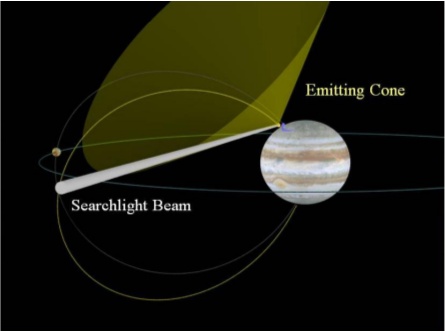
\includegraphics[width=8cm]{images/12}
\caption{A searchlight beam model of Jupiter's decametric radio emissions \citep{imai-08}}
\label{fig:decametric_emissions_searchlight}
\end{figure}
%

%
\begin{figure}[here]
\centering
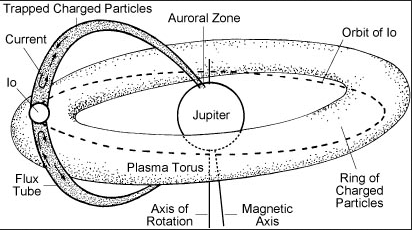
\includegraphics[width=8cm]{images/13}
\caption{Io Flux Tube and the Plasma Torus \citep{lang-10}}
\label{fig:io_flux_tube_plasma_torus}
\end{figure}
%

%
\begin{figure}[here]
\centering
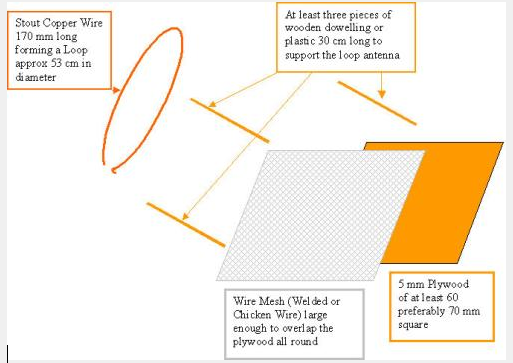
\includegraphics[width=8cm]{images/14}
\caption{21 MHz Shortwave Loop Antenna Radio Telescope Design \citep{greef-12}}
\label{fig:loop_antenna_design_a}
\end{figure}
%

%
\begin{figure}[here]
\centering
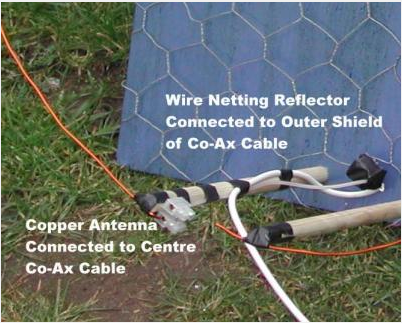
\includegraphics[width=8cm]{images/16}
\caption{21 MHz Shortwave Loop Antenna Radio Telescope Design \citep{greef-12}}
\label{fig:loop_antenna_design_b}
\end{figure}
%

%
\begin{figure}[here]
\centering
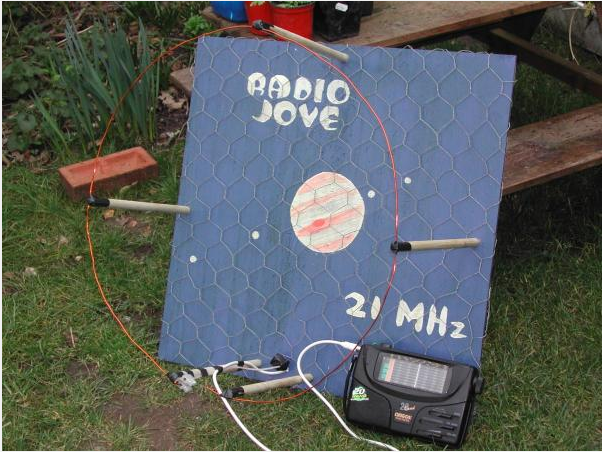
\includegraphics[width=8cm]{images/15}
\caption{21 MHz Shortwave Loop Antenna Radio Telescope Design \citep{greef-12}}
\label{fig:loop_antenna_design_c}
\end{figure}
%

%
\begin{figure}[here]
\centering
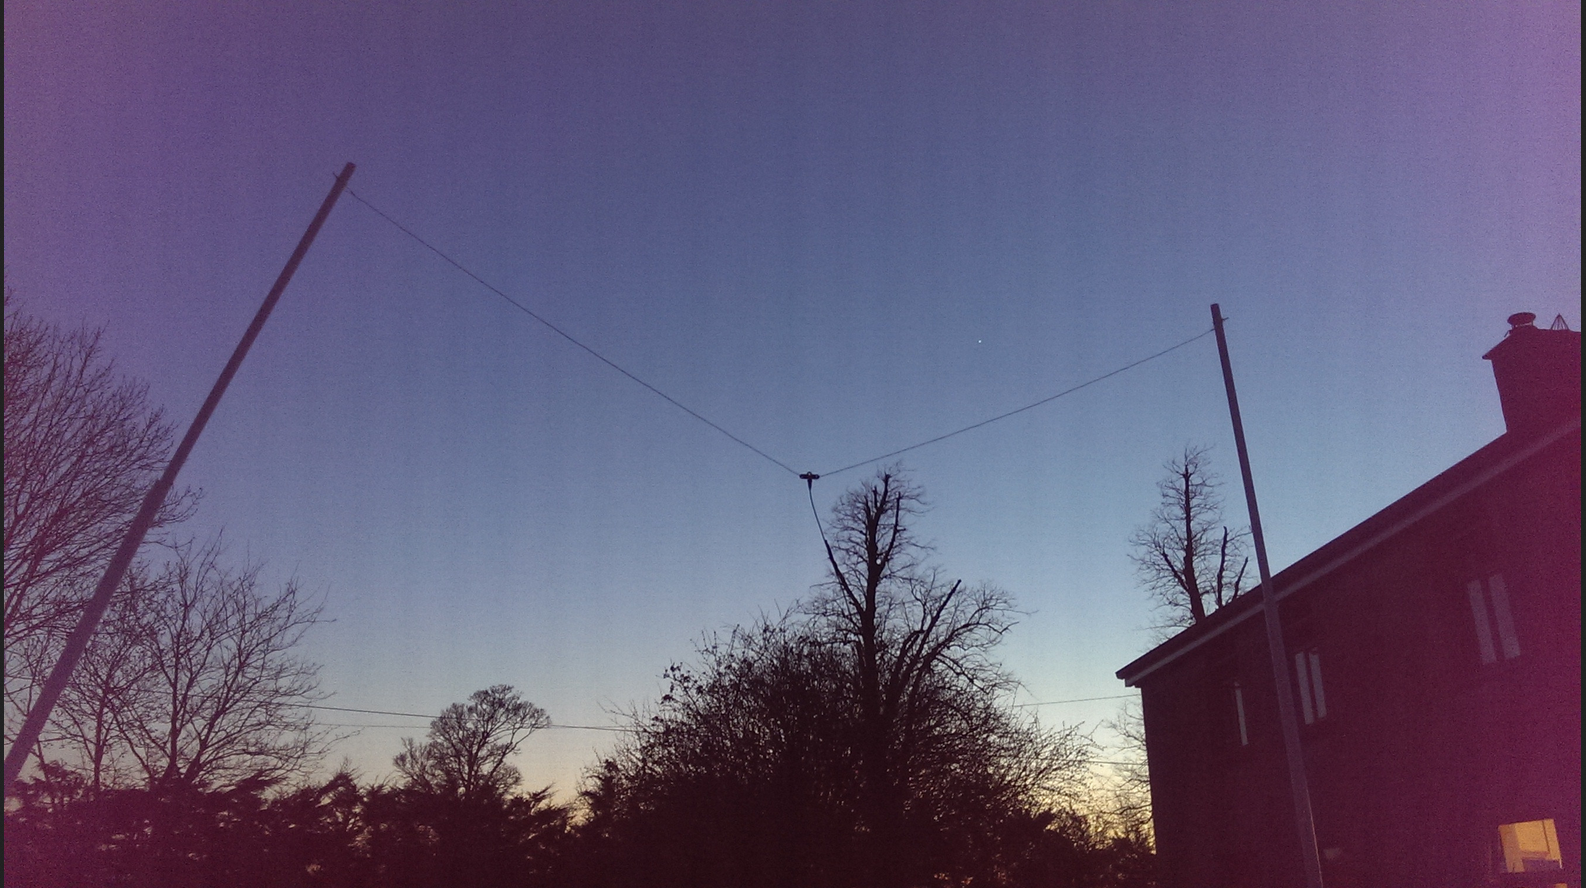
\includegraphics[width=8cm]{images/32}
\caption{Dual Dipole Antenna Deployment}
\label{fig:dual_dipole_deployed}
\end{figure}
%

%
\begin{figure}[here]
\centering
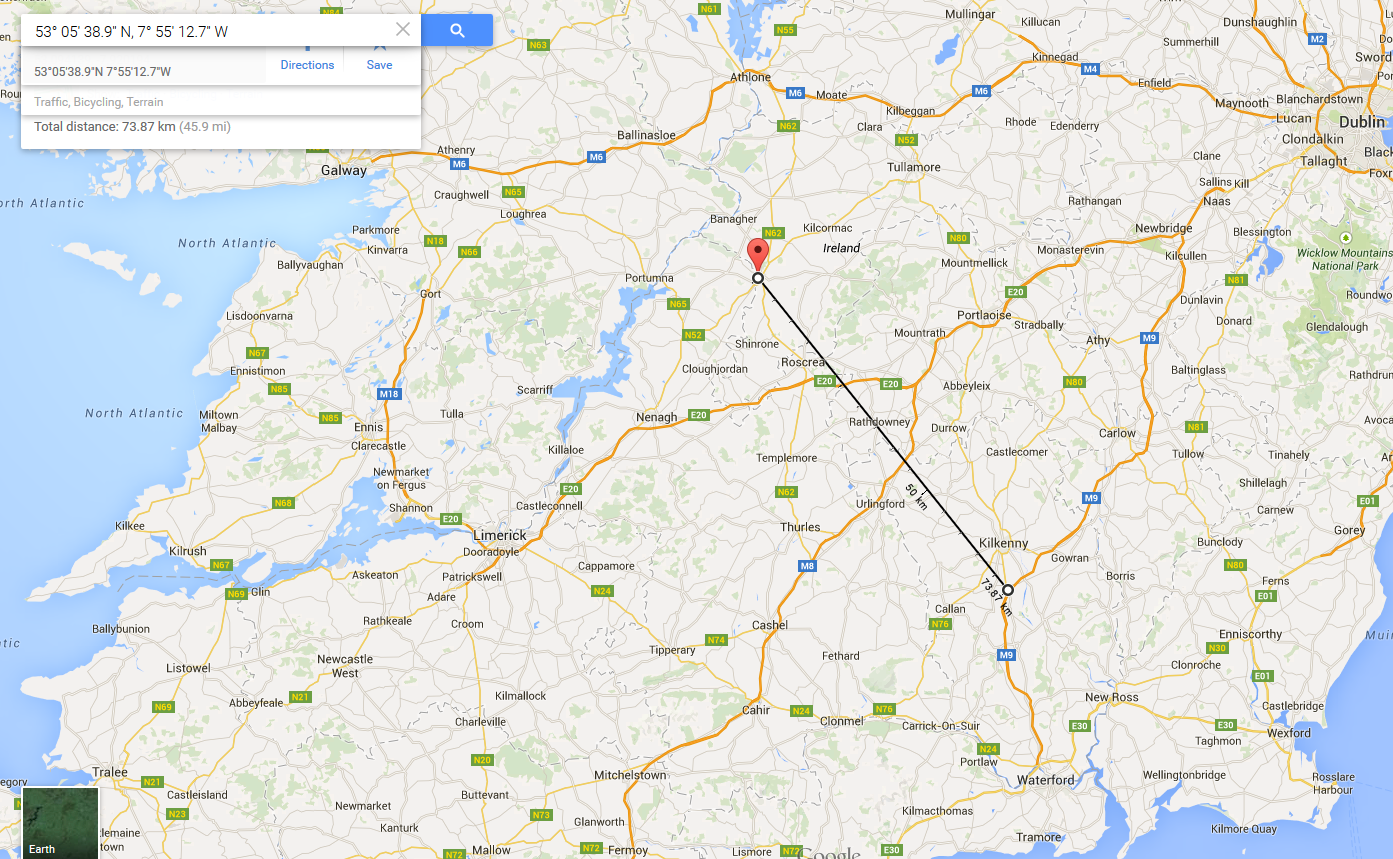
\includegraphics[width=8cm]{images/36}
\caption{Distance between the Birr and Kilkenny site survey}
\label{fig:site_survey_birr_kilkenny_distance}
\end{figure}
%

%
\begin{figure}[here]
\centering
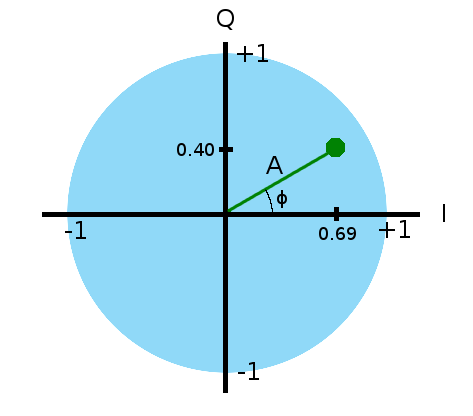
\includegraphics[width=8cm]{images/47}
\caption{I/Q Samples Polar Plot \citep{kuisma-14}}
\label{fig:kuisma-iq-polar}
\end{figure}
%

%
\begin{figure}[here]
\centering
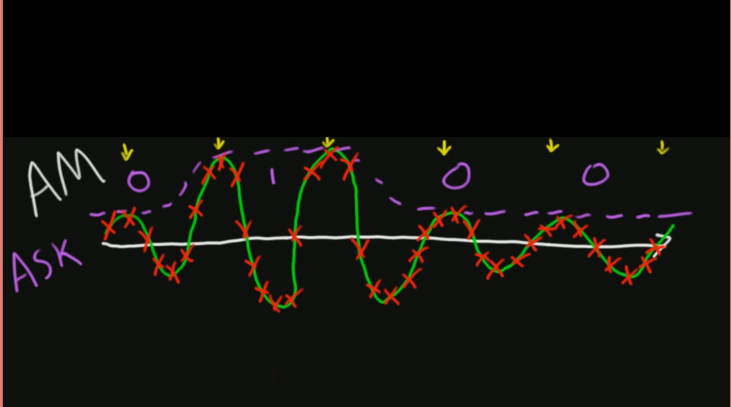
\includegraphics[width=8cm]{images/46}
\caption{Sampling an Analogue Amplitude Modulation Signal \citep{ossmann-15-c}}
\label{fig:ossmann_am_demodulation}
\end{figure}
%

%
\begin{figure}[here]
\centering
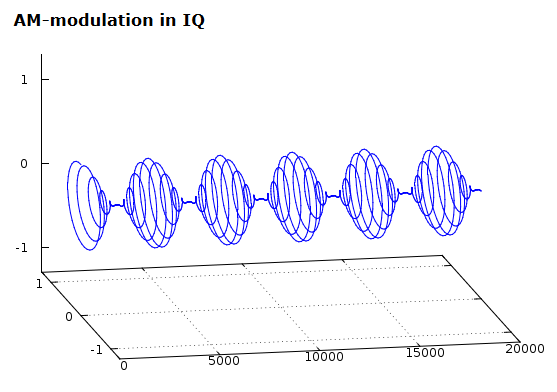
\includegraphics[width=8cm]{images/49}
\caption{I/Q Sample Polar Plot of an AM Modulated Signal \citep{kuisma-14}}
\label{fig:kuisma-iq-am-helix}
\end{figure}
%

%
\begin{figure}[here]
\centering
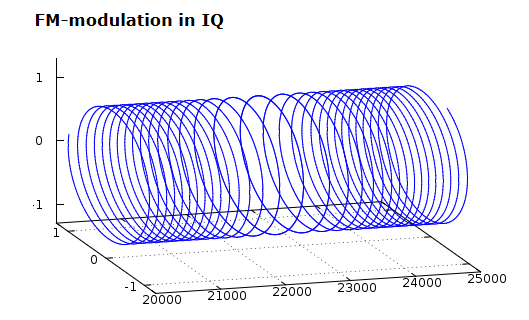
\includegraphics[width=8cm]{images/50}
\caption{I/Q Sample Polar Plot of an FM Modulated Signal \citep{kuisma-14}}
\label{fig:kuisma-iq-fm-helix}
\end{figure}
%

%
\begin{figure}[here]
	\centering
	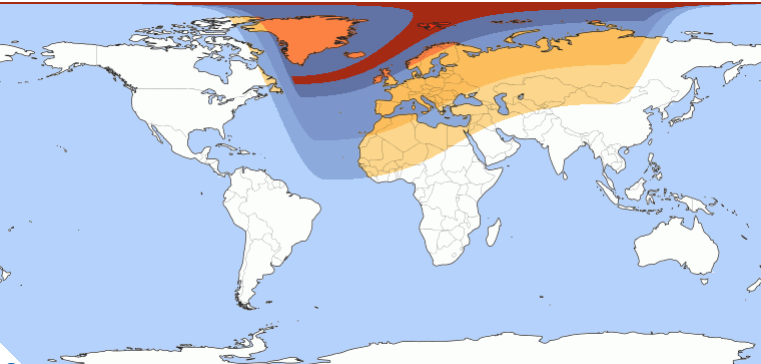
\includegraphics[width=8cm]{images/41}
	\caption{Partial Solar Eclipse 20th March 2015}
	\label{fig:solar_eclipse_scale}
\end{figure}
%


%
\bibliographystyle{plainnat}
\bibliography{bibliography/bibtex}
\addcontentsline{toc}{chapter}{Bibliography}
%

\end{document}


